\begin{enumerate}[label=\thesubsection.\arabic*,ref=\thesubsection.\theenumi]
\item 
Find the area between the curves $y=x$ and $y=x^2$.
\\
\solution
\label{chapters/12/8/3/2}
	\begin{figure}[H]
		\centering
 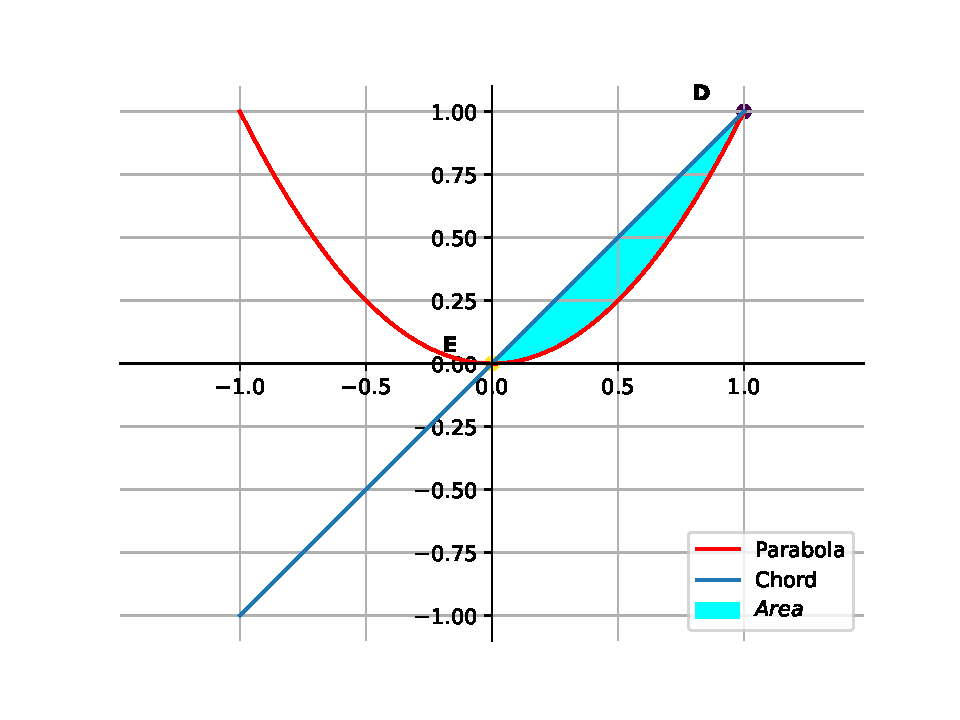
\includegraphics[width=0.75\columnwidth]{chapters/12/8/3/2/figs/fig.pdf}
		\caption{}
		\label{fig:12/8/3/2}
  	\end{figure}
The given curve  can be expressed as a conic with parameters
\begin{align}
	\vec{V} &= \myvec{1 & 0\\0 & 0}, \vec{u} = \myvec{0 \\-\frac{1}{2}}, f = 0
	\end{align}
The given line parameters are
\begin{align}
\vec{h} = \myvec{0 \\0}, \vec{m}=\myvec{1\\1}
\end{align}
Substituting the given parameters in 
\eqref{eq:tangent_roots},
\begin{align}
\vec{x}_1=\myvec{0\\0}, \vec{x}_2=\myvec{1\\1}.
\end{align}
From  
		\figref{fig:12/8/3/2},
the area bounded by the curve $y=x^2$ and line $y=x$ is given by
\begin{align}
	\int_{0}^{1} \brak{x 
	-\frac{x^2}{2}} \,dx = \frac{1}{6}
\end{align}

\item 
Find the area of the region bounded by the curve $y^2=x$ and the lines $x=1$ and $x=4$ and the axis in the first quadrant.
\label{chapters/12/8/1/1}
	\\
	\solution
	\begin{figure}[H]
		\centering
 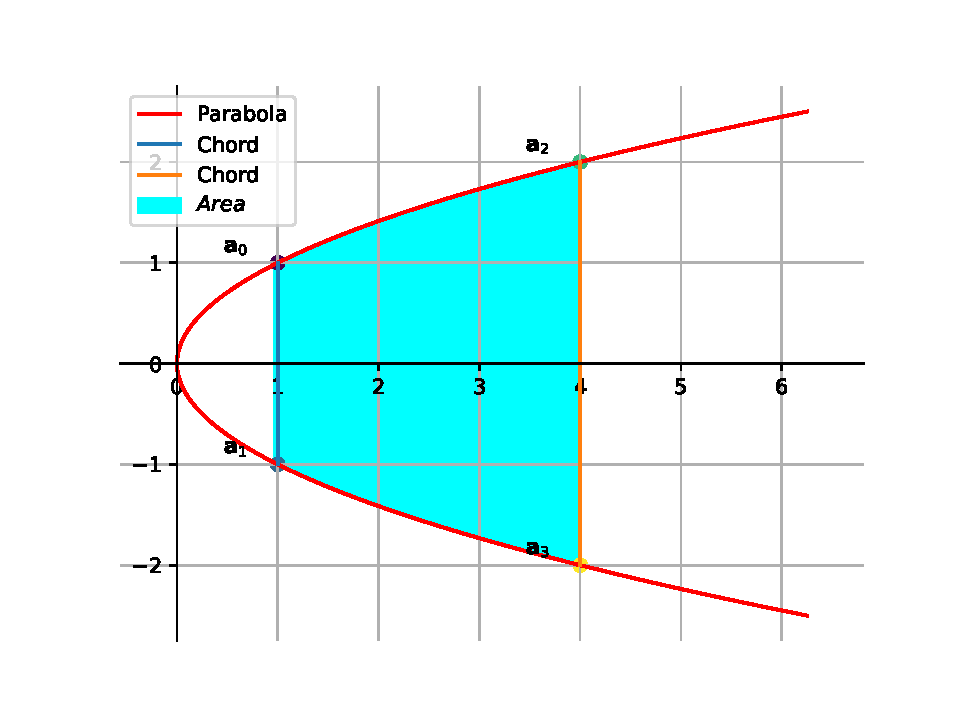
\includegraphics[width=0.75\columnwidth]{chapters/12/8/1/1/figs/fig.pdf}
		\caption{}
		\label{fig:12/8/1/1}
  	\end{figure}

The parameters of the conic are
\begin{align}
	\vec{V} = \myvec{0 & 0\\0 & 1},
	\vec{u} = -\frac{1}{2}\myvec{ 1\\0},
	f = 0
	%\\
\end{align}
\iffalse
The point of intersection of the lines $x=1$ and $x=4$ to the parabola is given by


The points of intersection of the line 
\begin{align}
	L: \quad \vec{x} = \vec{h} + \kappa \vec{m} \quad \kappa \in \mathbf{R}
\label{eq:conic_tangent}
\end{align}
with the conic section are given by
\begin{align}
\vec{x}_i = \vec{h} + \kappa_i \vec{m}
\label{eq:conic_tangent_pts}
\end{align}
%
where
{\tiny
\begin{multline}
\kappa_i = \frac{1}
{
\vec{m}^T\vec{V}\vec{m}
}
\lbrak{-\vec{m}^T\brak{\vec{V}\vec{h}+\vec{u}}}
\\
\pm
\rbrak{\sqrt{
\sbrak{
\vec{m}^T\brak{\vec{V}\vec{h}+\vec{u}}
}^2
-
\brak
{
\vec{h}^T\vec{V}\vec{h} + 2\vec{u}^T\vec{h} +f
}
\brak{\vec{m}^T\vec{V}\vec{m}}
}
}
\label{eq:tangent_roots}
\end{multline}
}
\fi
For the line $x-1=0$, the parameters are  
\begin{align}
	\vec{h}_2=\myvec{1\\0},
	\vec{m}_2=\myvec{0\\1}
\end{align}
Substituting from the above in 
\eqref{eq:tangent_roots},
\begin{align}
\kappa_i=1,-1
\end{align}
yilelding 
the points of intersection 
\begin{align}
	\vec{a}_0=\myvec{1\\1},
	\vec{a}_1=\myvec{1\\-1}
\end{align}
Similarly, 
for the line $x-4=0$ 
\begin{align}
\vec{q_1}=\myvec{4\\0},
\vec{m_1}=\myvec{0\\1}
\end{align}
yielding
\begin{align}
\kappa_i=2,-2
\end{align}
from which, the points of 
intersection are
\begin{align}
\vec{a_3}=\myvec{4\\2},
\vec{a_2}=\myvec{4\\-2}
\end{align}
		See \figref{fig:12/8/1/1}.
Thus, 
the area of the parabola in between the lines $x=1$ and $x=4$ is given by
\begin{align}
\int_{0}^{4} \ \sqrt{x} \,dx-\int_{0}^{1} \ \sqrt{x} \,dx
=14/3
\end{align}

\item 
Find the area of the region bounded by the curve $y^2=9x$ and the lines $x=2$ and $x=4$ and the axis in the first quadrant.
\item Find the area of the region bounded by ${x}^2
= 4{y}$, ${y} = 2$, ${y} = 4$ and the y-axis in the
first quadrant.
\label{chapters/12/8/1/3}
\item Find the area of the region bounded by the ellipse \(\frac{{x}^2}{16}\ + \frac{{y}^2}{9} = 1\)
\label{chapters/12/8/1/4}
\item Find the area of the region bounded by the ellipse \(\frac{{x}^2}{4}\ + \frac{{y}^2}{9} = 1\)
\label{chapters/12/8/1/5}
\item 
		  Find the area of the region in the first quadrant enclosed by the x-axis, line $x=\sqrt{3}y$ and circle $x^2+y^2=4$.
		  \\
		  \solution
\label{chapters/12/8/1/6}
	\begin{figure}[H]
		\centering
 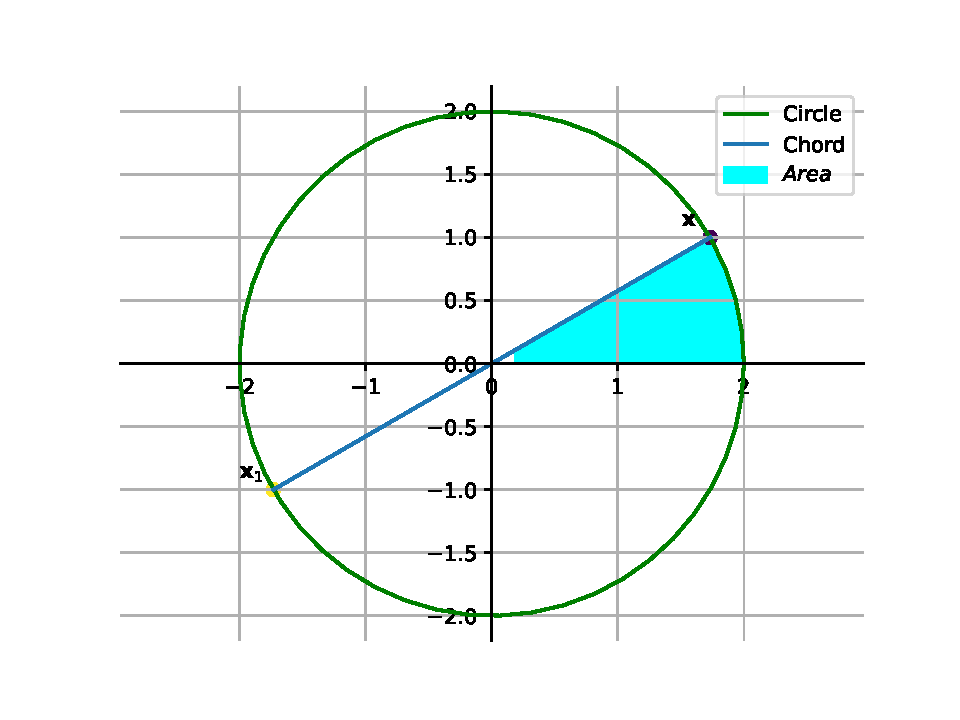
\includegraphics[width=0.75\columnwidth]{chapters/12/8/1/6/figs/fig.pdf} 
		\caption{}
		\label{fig:12/8/1/6}
  	\end{figure}
  From the given information, the parameters of the  circle and line are
                      \begin{align}
			      f= -4, \vec{u}=\vec{0}, \vec{V}=\vec{I}, \vec{m}=\myvec{1 \\ \sqrt{3}}, \vec{h} = \vec{0}
		\label{eq:12/8/1/6}
                    \end{align}                                                                              
Substituting		    the above parameters in  
\eqref{eq:tangent_roots},
	  \begin{align}                                                                               
		  \kappa= \sqrt{3}
	  \end{align}
	  yielding  
the desired point of intersection as                                               
\begin{align}
	\vec{x} = \myvec{\sqrt{3} \\ 1}                               
\end{align}
Note that we have chosen only the point of intersection in the first quadrant as shown in 
		\figref{fig:12/8/1/6}.
From
		\eqref{eq:12/8/1/6},
		the angle between the given line and the $X$ axis is
\begin{align}
	\theta=30\degree
\end{align} 
and
the area of the sector is 
\begin{align}
	{\frac{\theta}{360}}\pi r^2=
	\frac{\pi}{3}
\end{align}

\item 
	Find the area of the smaller part of the circle $x^2+y^2=a^2 $ cut off by the line $x=\frac{a}{\sqrt{2}}$.
	\\
	\solution
\label{chapters/12/8/1/7}
\begin{enumerate}[label=\thesubsection.\arabic*.,ref=\thesubsection.\theenumi]
\item STATEMENT-1: The curve $y=\frac{-x^2}{2}+x+1$ is symmetric with respect to the line $x=1$.
	\\
STATEMENT-2: A Parabola is symmetric about its axis.
\hfill(2007)
			\begin{multicols}{2}
\begin{enumerate}
    \item Statement-1 is True,Statement-2 is True;Statement-2 is a correct explanation for Statement-1\item  Statement-1 is True,Statement-2 is True;Statement-2 is NOT a correct explanation for Statement-1\item Statement-1 is True,Statement-2 is False\item Statement-1 is False,Statement-2 is True
\end{enumerate}\end{multicols}
\item A parabola has the origin as its focus and $x=2$ as the directrix. Then the vertex of the parabola is at\hfill(2009)
	\begin{multicols}{4}
\begin{enumerate}
    \item $\brak{0,2}$
    \item $\brak{1,0}$
    \item $\brak{0,1}$
    \item $\brak{2,0}$
\end{enumerate}\end{multicols}
\item The ellipse $x^2+y^2 = 4$ is inscribed in a rectangle aligned with the coordinate axes, which in turn is inscribed in another ellipse that passes through the point$\brak{4,0}$. Then the equation of the ellipse is:\hfill(2009)
	\begin{multicols}{2}
\begin{enumerate}
    \item $x^2+12y^2+16$
    \item $4x^2+48y^2=48$
    \item $4x^2+64y^2=48$
    \item $x^2+16y^2=16$
\end{enumerate}\end{multicols}
\item Equation of the ellipse whose axes are the coordinates and which passes through the point $\brak{-3,1}$ and has eccentricity $\sqrt{\frac{2}{5}}$ is\hfill(2011)
	\begin{multicols}{2}
\begin{enumerate}
    \item $5x^2+3y^2-48=0$
    \item $3x^2+5y^2-15=0$
    \item $5x^2+3y^2-32=0$
    \item $3x^2+5y^2-32=0$
\end{enumerate}\end{multicols}
\item An ellipse is drawn by taking a diameter of the circle $(x-1)^2+y^2=1$ as its semi minor axis and a diameter of the circle $x^2+(y-2)^2=4$ as semi-major axis. If the centre of the ellipse is at the origin and its axes are the coordinate axes, then the equation of the ellipse is 

\hfill(2012)
		\begin{multicols}{2}
\begin{enumerate}
    \item $4x^2+y^2=4$ 
    \item $x^2+4y^2=8$
    \item $4x^2+y^2=8$
    \item $x^2+4y^2=1$
\end{enumerate}\end{multicols}
\item The equation of the circle passing through the foci of the ellipse $\frac{x^2}{16}+\frac{y^2}{9}=1$, and having centre at $\brak{0,3}$ is

\hfill( 2013)
			\begin{multicols}{2}
\begin{enumerate}
    \item $x^2+y^2-6y-7=0$
    \item $x^2+y^2-6y+7=0$
    \item $x^2+y^2-6y-5=0$
    \item $x^2+y^2-6y+5=0$
\end{enumerate}\end{multicols}
\item Let $\vec{O}$ be the vertex and $\vec{Q}$ be any point on the parabola, $x^2=8y$. If the point $\vec{P}$ divides the line segment $OQ$ internally in the ratio \brak{1:3}, then the locus of $\vec{P}$ is

\hfill( 2015)
				\begin{multicols}{4}
\begin{enumerate}
    \item $y^2=2x$
    \item $x^2=2y$
    \item $x^2=y$
    \item $y^2=x$
\end{enumerate}\end{multicols}
\item Let $\vec{P}$ be the point on the parabola, $y^2=8x$ which is a minimum distance from the centre $\vec{C}$ of the circle, passing through $\vec{C}$ and having its centre at $\vec{P}$ is

\hfill( 2016)
					\begin{multicols}{2}
\begin{enumerate}
    \item $x^2+y^2-\frac{x}{4}+2y-24=0$ 
    \item $x^2+y^2-4x+9y+18=0$ 
    \item $x^2+y^2-4x+8y+12=0$
    \item $x^2+y^2-x+4y-12=0$
\end{enumerate}\end{multicols}
\item The eccentricity of the hyperbola whose length of the latus rectum is equal to $8$ and the length of its conjugate axis is equal to half of the distance between its foci, is 

\hfill(2016)
						\begin{multicols}{2}
\begin{enumerate}
    \item $\frac{2}{\sqrt{3}}$
    \item $\sqrt{3}$
    \item $\frac{4}{3}$
    \item $\frac{4}{\sqrt{3}}$
\end{enumerate}\end{multicols}

\item Match the conics in column 1 with the statements/expressions in column 2\hfill{(2009)}

\begin{multicols}{2}
\textbf{Column I}
\begin{enumerate}
    \item  Circle
    \item  Parabola
    \item  Ellipse 
    \item  Hyperbola  
\end{enumerate} 
\columnbreak
\textbf{Column II}
\begin{enumerate}
	\item The locus of the point ${(h,k)}$ for which the line $hx + ky =1$ touches the circle $x^2 + y^2 = 4$
    \item Points z in the complex plane satisfying $|z + 2|- |z - 2|= \pm 3$
    \item Points of the conic have parametric representations $x=\sqrt{3}
	    \brak{\frac{1 - t^2}{1 + t^2}}$, $ y = \frac{2t}{1 + t^2}$

    \item The eccentricity of the conic lies in the interval $1 \leq x < \infty$

\end{enumerate}
\end{multicols}


 \item Let $H : \frac{x^2}{a^2}-\frac{y^2}{b^2}= 1$, where $a>b>0$, be a hyperbola in $XY$-plane whose conjugate axis $LM$ subtends an angle of $60\degree$ at one of its vertices $\vec{N}$. Let the area of the triangle $LMN$ be 4$\sqrt{3}$.
Match the following.
\begin{multicols}{2}
\textbf{List 1}
\begin{enumerate}
    \item The length of the conjugate axis of $H$ is
    \item The eccentricity of $H$ is
    \item The distance between the foci of $H$ is
    \item The length of the latus rectum of $H$ is
\end{enumerate}
\columnbreak
\textbf{List 2}
\begin{enumerate}
    \item 8
    \item $\frac{4}{\sqrt{3}}$
    \item $\frac{2}{\sqrt{3}}$
    \item 4
\end{enumerate}
\end{multicols}
\item If $\vec{P}=\brak{x,y}$, $\vec{F}_{1}=\brak{3,0}$, $\vec{F}_{2}=\brak{-3,0}$ and $16x^2+25y^2=400$, then ${PF}_{1}+{PF}_{2}$ equals \hfill(1998)
	\begin{multicols}{4}
	\begin{enumerate}
		\item $8$
		\item $6$
		\item $10$
		\item $12$
	\end{enumerate}\end{multicols}

\item Let a hyperbola passes through the focus of the ellipse $\frac{x^2}{25}+\frac{y^2}{16}=1$. The transverse and conjugate axes of this hyperbola coincide with the major and minor axes of the given ellipse, also the product of eccentricities of given ellipse and hyperbola is $1$, then \hfill (2006)
	\begin{multicols}{2}
	\begin{enumerate}
		\item the equation of hyperbola is $\frac{x^2}{9}-\frac{y^2}{16}=1$
		\item the equation of hyperbola is $\frac{x^2}{9}-\frac{y^2}{25}=1$
		\item focus of hyperbola is $\brak{5,0}$
		\item vertex of hyperbola is $\brak{5\sqrt{3},0}$
	\end{enumerate}\end{multicols}

\item Let $\vec{P}\brak{x_{1}, y_{1}}$ and $\vec{Q}\brak{x_{2},y_{2}}$, $y_{1}<0,y_{2}<0$, be the end points of the latus rectum of the ellipse $x^2+4y^2=4$. The equations of parabolas with latus rectum ${PQ}$ are \hfill(2008)
	\begin{multicols}{2}
	\begin{enumerate}
		\item $x^2+2\sqrt{3}y=3+\sqrt{3}$
		\item $x^2-2\sqrt{3}y=3+\sqrt{3}$
			\columnbreak
		\item $x^2+2\sqrt{3}y=3-\sqrt{3}$
		\item $x^2-2\sqrt{3}y=3-\sqrt{3}$
	\end{enumerate}\end{multicols}

\item In a triangle ${ABC}$ with fixed base ${BC}$, the vertex $\vec{A}$ moves such that
	$$\cos{B}+\cos{C}=4\sin^2{\frac{A}{2}}.$$
		If $a,b$ and $c$ denote the lengths of the sides of the triangle opposite to the angles $A,B$ and $C$, respectively, then \hfill(2009)\\
		\begin{enumerate}
			\item $b+c=4a$
			\item $b+c=2a$
			\item locus of the point $\vec{A}$ is an ellipse
			\item locus of the point $\vec{A}$ is a pair of straight lines
		\end{enumerate}

	\item Let the eccentricity of the hyperbola $\frac{x^2}{a^2}-\frac{y^2}{b^2}=1$ be reciprocal to that of the elipse $x^2+4y^2=4$. If the hyperbola
	passes through a focus of the elipse, then 
		\hfill(2011)
		 \begin{enumerate}
			\item the equation of the hyperbola is $\frac{x^2}{3}-\frac{y^2}{2}=1$
			\item a focus of the hypebola is $(2,0)$
			\item the eccentricity of the hyperbola is $\sqrt{\frac{5}{3}}$
			\item the equation of the hyperbola is $x^2-3y^2=3$
		 \end{enumerate}
	\item Let $\vec{P}$ and $\vec{Q}$ be distinct points on the parabola $y^2=2x$ such 
		that a circle with $PQ$ as diameter passes through the vertex
		$\vec{O}$ of the parabola. If $\vec{P}$ lies in the first quadrant and the area
		of the triangle  \(\Delta \)$OPQ$ is 3$\sqrt{2}$, then which of the following is
		(are) the coordinates of $\vec{P}$?  
		\hfill(2015)
				\begin{multicols}{4}
		 \begin{enumerate}
			\item $ \brak{4,2\sqrt{2}}$
			\item $\brak{9,3\sqrt{2}}$
			\item $ \brak{\frac{1}{4},\frac{1}{\sqrt{2}}}$
			\item  $ \brak{1,\sqrt{2}}$
		 \end{enumerate}\end{multicols}
    \item The equation $\frac{x^2}{1-r}-\frac{y^2}{1+r}=1,r > 1$
represents
          \hfill  \brak{1981}
					\begin{multicols}{2}
\begin{enumerate}
    \item an ellipse    \item       a hyperbola
   \item a circle     \item    none of there 
\end{enumerate}\end{multicols}
\item Each of the four inequalities give below defines a region in $xy$ plane.One of these four regions does not have the following property.For any two points   $\brak{\frac{x_1+x_2}{2},\frac{y_1+y_2}{2}}$   is also in region.The inequality defining this region is:
         \hfill \brak{1981}
						\begin{multicols}{2}
\begin{enumerate}
    \item $x^2+2y^2\le1$
    \item Max $\abs{x},\abs{y}$ $\le1$
    \item $x^2-y^2\le1$
    \item $y^2-x\le0$
\end{enumerate}\end{multicols}
\item The equation $2x^2+3y^2-8x-18y+35=k$ represents
        \hfill \brak{1994}
							\begin{multicols}{2}
\begin{enumerate}
    \item no locus if $k\textless0$
    \item an ellipse if $k\textless0$
    \item a point if $k=0$
    \item a hyperbola if $k\textgreater0$ 
\end{enumerate}\end{multicols}
\item Let $E$ be the ellipse $\frac{x^2}{9}+\frac{y^2}{4}=1$ and $C$ be the circle $x^2+y^2=9$. Let $\vec{P}$ and $\vec{Q}$ be the points $\brak{1,2}$ and $\brak{2,1}$ respectively.Then
        \hfill \brak{1994}
								\begin{multicols}{2}
\begin{enumerate}
    \item $\vec{Q}$ lies inside $C$ but outside $E$
    \item $\vec{Q}$ lies outside both $C$ and $E$
    \item $\vec{P}$ lies inside both $C$ and $E$
    \item $\vec{P}$ lies inside $C$ but outside $E$ 
\end{enumerate}\end{multicols}
\item The radius of the circle passing through the foci of the ellipse $\frac{x^2}{16}+\frac{y^2}{9}=1$ and having its centre at $\brak{0,3}$ is
       \hfill \brak{1995}
									\begin{multicols}{4}
\begin{enumerate}
    \item $4$
    \item $3$
    \item $\sqrt{\frac{1}{2}}$
    \item $\frac{7}{2}$
\end{enumerate}\end{multicols}
\item The curve described parametrically by $x=t^2+t+1$, $y=t^2-t+1$ represents
     \hfill\brak{1999}
										\begin{multicols}{2}
\begin{enumerate}
    \item a pair of straight lines
    \item an ellipse
    \item a parabola
    \item a hyperbola
\end{enumerate}\end{multicols}
\item If the line $x-1=0$ is the directrix of parabola $y^2-kx+8=0$, then one of the values of $K$ is
      \hfill\brak{2000}
											\begin{multicols}{2}
\begin{enumerate}
    \item $\frac{1}{8}$
    \item $8$
    \item $4$
    \item $\frac{1}{4}$ 
\end{enumerate}\end{multicols}
    \item The equation of the directrix of the parabola $y^2+4y+4x+2=0$ is 
     \hfill \brak{2001}
												\begin{multicols}{2}
\begin{enumerate}
    \item $x=-1$
    \item $x=1$
    \item $x=-\frac{3}{2}$
     \item $x=\frac{3}{2}$
\end{enumerate}\end{multicols}
\item The locus of the mid-point of the line segment joining the focus to a moving point on the parabola $y^{2} = 4ax$ is another parabola with directrix \hfill{(2002)}
\begin{multicols}{4}
 \begin{enumerate}
    \item x=-a
    \item x=-a/2
    \item x=a
    \item x=a/2
 \end{enumerate}
\end{multicols}
\item For hyperbola $\frac{x^{2}}{\cos^{2}\alpha}-\frac{y^{2}}{\sin^{2}\alpha}=1$ which of the following remains constant with change in $\alpha$
\hfill{(2003)}
\begin{multicols}{2}
\begin{enumerate}
    \item abscissae of vertices
    \item abscissae of foci
    \item eccentricity
    \item directrix
\end{enumerate}
\end{multicols}
\item The axis of the parabola is along the line $y=x$ and the distance of its vertex and focus from  origin are $\sqrt2$ and $2\sqrt2$  respectively. If the vertex and focus both lie in the first quadrant,then the equation of the parabola is \hfill{(2006)}
\begin{multicols}{2}
\begin{enumerate}
    \item $(x+y)^{2}=(x-y-2)$
    \item $(x-y)^{2}=(x+y-2)$
    \item $(x-y)^{2}=4(x+y-2)$
    \item $(x-y)^{2}=8(x+y-2)$
\end{enumerate}
\end{multicols}
\item A hyperbola, having the transverse axis of length $2\sin\theta$, is confocal with the ellipse $3x^{2}+4y^{2}=12$. Then its equation is \hfill{(2007)}
	\begin{multicols}{2}
\begin{enumerate}
    \item ${x^{2}\cosec^{2}\theta}-{y^{2}\sec^{2}\theta=1}$
    \item $x^{2}\sec^{2}\theta-y^{2}\cosec^{2}\theta=1$
    \item $x^{2}\sin^{2}\theta-y^{2}\cos^{2}\theta=1$
    \item $x^{2}\cos^{2}\theta-y^{2}\sin^{2}\theta=1$
\end{enumerate}\end{multicols}
\item Let $a$ and $b$ be non-zero real numbers. Then, the equation $(ax^{2}+by^{2}+c)(x^{2}-5xy+6y^{2}=0)$ represents \hfill{(2008)}
\begin{enumerate}
    \item four straight lines, when $c=0$ and $a, b$ are of the same sign.
    \item two straight lines and a circle, when $a=b$,and $c$ is of sign opposite to that of $a$.
    \item two straight lines and a hyperbola, when $a$ and $b$ are of the same sign and $c$ is of opposite to that of $a$.
    \item a circle and an ellipse, when $a$ and $b$ are of the same sign and $c$ is of sign opposite to that of $a$.
\end{enumerate}
\item Consider a branch of the hyperbola $x^{2}-2y^{2}-2\sqrt{2}x-4\sqrt{2}y-6=0$ with vertex at a point  $\vec{A}$. Let  $\vec{B}$  be one of the end points of its latus rectum. If $\vec{C}$ is the focus of the hyperbola nearest to the point  $\vec{A}$, then the area of the triangle $ABC$ is \hfill{(2008)}
\begin{multicols}{4}
\begin{enumerate}
    \item $1-\sqrt{\frac{2}{3}}$
    \item $\sqrt{\frac{3}{2}}-1$
    \item $1+\sqrt{\frac{2}{3}}$
    \item $\sqrt{\frac{3}{2}}+1$
\end{enumerate}
\end{multicols}
\item The line passing through the extremity $\vec{A}$ of the major axis and extremity $\vec{B}$ of the minor axis of the ellipse $x^{2}+9y^{2}=9$ meets its auxillary circle at the point $\vec{M}$. Then the area of the triangle with the vertices at $\vec{A}$, $\vec{M}$ and the origin $\vec{O}$ is \hfill{(2009)}
\begin{multicols}{4}
\begin{enumerate}
    \item $\frac{31}{10}$
    \item $\frac{29}{10}$
    \item $\frac{21}{10}$
    \item $\frac{27}{10}$
\end{enumerate}\end{multicols}
	%	
\item The locus of the orthocentre of the triangle formed by the lines
		
			$$\brak{1+p}x-py+p\brak{1+p}=0,$$
			$$\brak{1+q}x-qy+q\brak{1+q}=0,$$
		and $y=0$, where $p \neq q$, is
		\hfill(2009)
		\begin{multicols}{4}
\begin{enumerate}
	\item a hyperbola
	\item a parabola
	\item an ellipse
	\item a straight line
\end{enumerate}\end{multicols}
%
	\item Let $\brak{x,y}$ be any point on the parabola $y^2=4x$. Let $\vec{P}$ be the point that divides the line segment from $\brak{0,0}$ to $\brak{x,y}$ in the ratio $1:3$. Then the locus of $\vec{P}$ is  \hfill(2011)
		\begin{multicols}{4}
		\begin{enumerate}
			\item $x^2=y$
			\item $y^2=2x$
				\columnbreak
			\item $y^2=x$
			\item $x^2=2y$
		\end{enumerate}\end{multicols}
%
	\item The ellipse $E_{1}$:$\frac{x^2}{9}+\frac{y^2}{4}=1$ is inscribed in a rectangle $\vec{R}$ whose sides are parallel to the coordinate axes. Another ellipse $E_{2}$ passing through the point $\brak{0,4}$ circumscribes the rectangle $\vec{R}$. The eccentricity of the ellipse $E_{2}$ is \hfill(2012)
%
		\begin{multicols}{4}
		\begin{enumerate}
			\item $\frac{\sqrt{2}}{2}$
			\item $\frac{\sqrt{3}}{2}$
				\columnbreak
			\item $\frac{1}{2}$
			\item $\frac{3}{4}$
		\end{enumerate}\end{multicols}
%
\item  Two sets $A$ and $B$ are as under:
$A=\cbrak{\brak{a,b}\in\mathbb{R}\times\mathbb{R}:\abs{a-5}<1\text{ and} \abs{b-5}<1}$
$B=\cbrak{\brak{a,b}\in\mathbb{R}\times\mathbb{R}:4(a-6)^2\text{+}9(b-5)^2\leq36}$
    \hfill{( 2018)}
			\begin{multicols}{2}
	\begin{enumerate}
		\item $A\subset B$ 
		\item $A\cap B$
		\item neither $A\subset B$ nor $B\subset A$
		\item $B\subset A$
	\end{enumerate}\end{multicols}
\item Axis of a parabola lies along $X$ axis. If its vertex and focus are at a distance $2$ and $4$ respectively from origin, on the positive $X$ axis then which of the following points does not lie on it? 
     \hfill{( 2018)} 
				\begin{multicols}{4}
	\begin{enumerate}
    		\item $\brak{5,2\sqrt6}$
    		\item $\brak{8,6}$
    		\item $\brak{6,4\sqrt2}$
    		\item $\brak{4,-4}$
	\end{enumerate}\end{multicols}
\item Let $0<\theta<\pi/2$. If the eccentricty of the hyperbola $\frac{x^2}{\cos^2{\theta}} - \frac{y^2}{\sin^2{\theta}} = 1$ is greater than $2$, then the length of its latus rectum lies in the interval
	\hfill{( 2019)}
					\begin{multicols}{4}
	\begin{enumerate}
    		\item $\brak{5,\infty}$
    		\item $\lbrak{\frac{3}{2}},\rsbrak{3}$
    		\item $\lbrak{2},\rsbrak{3}$ 
    		\item $\lbrak{1},\rsbrak{\frac{3}{2}}$
	\end{enumerate} \end{multicols}
\item  The equation of the locus of the point whose distances from the point $\Vec{P}$ and the line $AB$ are equal, is

	\begin{multicols}{2}
\begin{enumerate}
     \item $9x^2+y^2-6xy-54x-62y+241=0$
     \item $x^2+9y^2+6xy-54x-62y-241=0$
     \item $9x^2+9y^2-6xy-54x-62y-241=0$
     \item $x^2+y^2-2xy+27x+31y-120=0$
\end{enumerate}\end{multicols}
\item Let $\vec{P}$ be a point on the ellipse $\frac{x^2}{a^2}+\frac{y^2}{b^2}=1$, $0<b<a$. Let the line parallel to the $X$ axis passing through $\vec{P}$ meet the circle $x^2+y^2=a^2$ at the point $\vec{Q}$ such that $\vec{P}$ and $\vec{Q}$ are on the same side of the $X$ axis. For two positive real numbers $r$ and $s$, find the locus of the point $\vec{R}$ on $PQ$ such that $PR
= r$ as $\vec{P}$ varies over the ellipse. \hfill\brak{2001}


	\end{enumerate}

\item 
The area between $x = y^2$ and $x = 4$ is divided into two equal parts by the line $x = a$, find the value of a.
\\
\solution
\label{chapters/12/8/1/8}
\begin{enumerate}[label=\thesubsection.\arabic*.,ref=\thesubsection.\theenumi]
\item STATEMENT-1: The curve $y=\frac{-x^2}{2}+x+1$ is symmetric with respect to the line $x=1$.
	\\
STATEMENT-2: A Parabola is symmetric about its axis.
\hfill(2007)
			\begin{multicols}{2}
\begin{enumerate}
    \item Statement-1 is True,Statement-2 is True;Statement-2 is a correct explanation for Statement-1\item  Statement-1 is True,Statement-2 is True;Statement-2 is NOT a correct explanation for Statement-1\item Statement-1 is True,Statement-2 is False\item Statement-1 is False,Statement-2 is True
\end{enumerate}\end{multicols}
\item A parabola has the origin as its focus and $x=2$ as the directrix. Then the vertex of the parabola is at\hfill(2009)
	\begin{multicols}{4}
\begin{enumerate}
    \item $\brak{0,2}$
    \item $\brak{1,0}$
    \item $\brak{0,1}$
    \item $\brak{2,0}$
\end{enumerate}\end{multicols}
\item The ellipse $x^2+y^2 = 4$ is inscribed in a rectangle aligned with the coordinate axes, which in turn is inscribed in another ellipse that passes through the point$\brak{4,0}$. Then the equation of the ellipse is:\hfill(2009)
	\begin{multicols}{2}
\begin{enumerate}
    \item $x^2+12y^2+16$
    \item $4x^2+48y^2=48$
    \item $4x^2+64y^2=48$
    \item $x^2+16y^2=16$
\end{enumerate}\end{multicols}
\item Equation of the ellipse whose axes are the coordinates and which passes through the point $\brak{-3,1}$ and has eccentricity $\sqrt{\frac{2}{5}}$ is\hfill(2011)
	\begin{multicols}{2}
\begin{enumerate}
    \item $5x^2+3y^2-48=0$
    \item $3x^2+5y^2-15=0$
    \item $5x^2+3y^2-32=0$
    \item $3x^2+5y^2-32=0$
\end{enumerate}\end{multicols}
\item An ellipse is drawn by taking a diameter of the circle $(x-1)^2+y^2=1$ as its semi minor axis and a diameter of the circle $x^2+(y-2)^2=4$ as semi-major axis. If the centre of the ellipse is at the origin and its axes are the coordinate axes, then the equation of the ellipse is 

\hfill(2012)
		\begin{multicols}{2}
\begin{enumerate}
    \item $4x^2+y^2=4$ 
    \item $x^2+4y^2=8$
    \item $4x^2+y^2=8$
    \item $x^2+4y^2=1$
\end{enumerate}\end{multicols}
\item The equation of the circle passing through the foci of the ellipse $\frac{x^2}{16}+\frac{y^2}{9}=1$, and having centre at $\brak{0,3}$ is

\hfill( 2013)
			\begin{multicols}{2}
\begin{enumerate}
    \item $x^2+y^2-6y-7=0$
    \item $x^2+y^2-6y+7=0$
    \item $x^2+y^2-6y-5=0$
    \item $x^2+y^2-6y+5=0$
\end{enumerate}\end{multicols}
\item Let $\vec{O}$ be the vertex and $\vec{Q}$ be any point on the parabola, $x^2=8y$. If the point $\vec{P}$ divides the line segment $OQ$ internally in the ratio \brak{1:3}, then the locus of $\vec{P}$ is

\hfill( 2015)
				\begin{multicols}{4}
\begin{enumerate}
    \item $y^2=2x$
    \item $x^2=2y$
    \item $x^2=y$
    \item $y^2=x$
\end{enumerate}\end{multicols}
\item Let $\vec{P}$ be the point on the parabola, $y^2=8x$ which is a minimum distance from the centre $\vec{C}$ of the circle, passing through $\vec{C}$ and having its centre at $\vec{P}$ is

\hfill( 2016)
					\begin{multicols}{2}
\begin{enumerate}
    \item $x^2+y^2-\frac{x}{4}+2y-24=0$ 
    \item $x^2+y^2-4x+9y+18=0$ 
    \item $x^2+y^2-4x+8y+12=0$
    \item $x^2+y^2-x+4y-12=0$
\end{enumerate}\end{multicols}
\item The eccentricity of the hyperbola whose length of the latus rectum is equal to $8$ and the length of its conjugate axis is equal to half of the distance between its foci, is 

\hfill(2016)
						\begin{multicols}{2}
\begin{enumerate}
    \item $\frac{2}{\sqrt{3}}$
    \item $\sqrt{3}$
    \item $\frac{4}{3}$
    \item $\frac{4}{\sqrt{3}}$
\end{enumerate}\end{multicols}

\item Match the conics in column 1 with the statements/expressions in column 2\hfill{(2009)}

\begin{multicols}{2}
\textbf{Column I}
\begin{enumerate}
    \item  Circle
    \item  Parabola
    \item  Ellipse 
    \item  Hyperbola  
\end{enumerate} 
\columnbreak
\textbf{Column II}
\begin{enumerate}
	\item The locus of the point ${(h,k)}$ for which the line $hx + ky =1$ touches the circle $x^2 + y^2 = 4$
    \item Points z in the complex plane satisfying $|z + 2|- |z - 2|= \pm 3$
    \item Points of the conic have parametric representations $x=\sqrt{3}
	    \brak{\frac{1 - t^2}{1 + t^2}}$, $ y = \frac{2t}{1 + t^2}$

    \item The eccentricity of the conic lies in the interval $1 \leq x < \infty$

\end{enumerate}
\end{multicols}


 \item Let $H : \frac{x^2}{a^2}-\frac{y^2}{b^2}= 1$, where $a>b>0$, be a hyperbola in $XY$-plane whose conjugate axis $LM$ subtends an angle of $60\degree$ at one of its vertices $\vec{N}$. Let the area of the triangle $LMN$ be 4$\sqrt{3}$.
Match the following.
\begin{multicols}{2}
\textbf{List 1}
\begin{enumerate}
    \item The length of the conjugate axis of $H$ is
    \item The eccentricity of $H$ is
    \item The distance between the foci of $H$ is
    \item The length of the latus rectum of $H$ is
\end{enumerate}
\columnbreak
\textbf{List 2}
\begin{enumerate}
    \item 8
    \item $\frac{4}{\sqrt{3}}$
    \item $\frac{2}{\sqrt{3}}$
    \item 4
\end{enumerate}
\end{multicols}
\item If $\vec{P}=\brak{x,y}$, $\vec{F}_{1}=\brak{3,0}$, $\vec{F}_{2}=\brak{-3,0}$ and $16x^2+25y^2=400$, then ${PF}_{1}+{PF}_{2}$ equals \hfill(1998)
	\begin{multicols}{4}
	\begin{enumerate}
		\item $8$
		\item $6$
		\item $10$
		\item $12$
	\end{enumerate}\end{multicols}

\item Let a hyperbola passes through the focus of the ellipse $\frac{x^2}{25}+\frac{y^2}{16}=1$. The transverse and conjugate axes of this hyperbola coincide with the major and minor axes of the given ellipse, also the product of eccentricities of given ellipse and hyperbola is $1$, then \hfill (2006)
	\begin{multicols}{2}
	\begin{enumerate}
		\item the equation of hyperbola is $\frac{x^2}{9}-\frac{y^2}{16}=1$
		\item the equation of hyperbola is $\frac{x^2}{9}-\frac{y^2}{25}=1$
		\item focus of hyperbola is $\brak{5,0}$
		\item vertex of hyperbola is $\brak{5\sqrt{3},0}$
	\end{enumerate}\end{multicols}

\item Let $\vec{P}\brak{x_{1}, y_{1}}$ and $\vec{Q}\brak{x_{2},y_{2}}$, $y_{1}<0,y_{2}<0$, be the end points of the latus rectum of the ellipse $x^2+4y^2=4$. The equations of parabolas with latus rectum ${PQ}$ are \hfill(2008)
	\begin{multicols}{2}
	\begin{enumerate}
		\item $x^2+2\sqrt{3}y=3+\sqrt{3}$
		\item $x^2-2\sqrt{3}y=3+\sqrt{3}$
			\columnbreak
		\item $x^2+2\sqrt{3}y=3-\sqrt{3}$
		\item $x^2-2\sqrt{3}y=3-\sqrt{3}$
	\end{enumerate}\end{multicols}

\item In a triangle ${ABC}$ with fixed base ${BC}$, the vertex $\vec{A}$ moves such that
	$$\cos{B}+\cos{C}=4\sin^2{\frac{A}{2}}.$$
		If $a,b$ and $c$ denote the lengths of the sides of the triangle opposite to the angles $A,B$ and $C$, respectively, then \hfill(2009)\\
		\begin{enumerate}
			\item $b+c=4a$
			\item $b+c=2a$
			\item locus of the point $\vec{A}$ is an ellipse
			\item locus of the point $\vec{A}$ is a pair of straight lines
		\end{enumerate}

	\item Let the eccentricity of the hyperbola $\frac{x^2}{a^2}-\frac{y^2}{b^2}=1$ be reciprocal to that of the elipse $x^2+4y^2=4$. If the hyperbola
	passes through a focus of the elipse, then 
		\hfill(2011)
		 \begin{enumerate}
			\item the equation of the hyperbola is $\frac{x^2}{3}-\frac{y^2}{2}=1$
			\item a focus of the hypebola is $(2,0)$
			\item the eccentricity of the hyperbola is $\sqrt{\frac{5}{3}}$
			\item the equation of the hyperbola is $x^2-3y^2=3$
		 \end{enumerate}
	\item Let $\vec{P}$ and $\vec{Q}$ be distinct points on the parabola $y^2=2x$ such 
		that a circle with $PQ$ as diameter passes through the vertex
		$\vec{O}$ of the parabola. If $\vec{P}$ lies in the first quadrant and the area
		of the triangle  \(\Delta \)$OPQ$ is 3$\sqrt{2}$, then which of the following is
		(are) the coordinates of $\vec{P}$?  
		\hfill(2015)
				\begin{multicols}{4}
		 \begin{enumerate}
			\item $ \brak{4,2\sqrt{2}}$
			\item $\brak{9,3\sqrt{2}}$
			\item $ \brak{\frac{1}{4},\frac{1}{\sqrt{2}}}$
			\item  $ \brak{1,\sqrt{2}}$
		 \end{enumerate}\end{multicols}
    \item The equation $\frac{x^2}{1-r}-\frac{y^2}{1+r}=1,r > 1$
represents
          \hfill  \brak{1981}
					\begin{multicols}{2}
\begin{enumerate}
    \item an ellipse    \item       a hyperbola
   \item a circle     \item    none of there 
\end{enumerate}\end{multicols}
\item Each of the four inequalities give below defines a region in $xy$ plane.One of these four regions does not have the following property.For any two points   $\brak{\frac{x_1+x_2}{2},\frac{y_1+y_2}{2}}$   is also in region.The inequality defining this region is:
         \hfill \brak{1981}
						\begin{multicols}{2}
\begin{enumerate}
    \item $x^2+2y^2\le1$
    \item Max $\abs{x},\abs{y}$ $\le1$
    \item $x^2-y^2\le1$
    \item $y^2-x\le0$
\end{enumerate}\end{multicols}
\item The equation $2x^2+3y^2-8x-18y+35=k$ represents
        \hfill \brak{1994}
							\begin{multicols}{2}
\begin{enumerate}
    \item no locus if $k\textless0$
    \item an ellipse if $k\textless0$
    \item a point if $k=0$
    \item a hyperbola if $k\textgreater0$ 
\end{enumerate}\end{multicols}
\item Let $E$ be the ellipse $\frac{x^2}{9}+\frac{y^2}{4}=1$ and $C$ be the circle $x^2+y^2=9$. Let $\vec{P}$ and $\vec{Q}$ be the points $\brak{1,2}$ and $\brak{2,1}$ respectively.Then
        \hfill \brak{1994}
								\begin{multicols}{2}
\begin{enumerate}
    \item $\vec{Q}$ lies inside $C$ but outside $E$
    \item $\vec{Q}$ lies outside both $C$ and $E$
    \item $\vec{P}$ lies inside both $C$ and $E$
    \item $\vec{P}$ lies inside $C$ but outside $E$ 
\end{enumerate}\end{multicols}
\item The radius of the circle passing through the foci of the ellipse $\frac{x^2}{16}+\frac{y^2}{9}=1$ and having its centre at $\brak{0,3}$ is
       \hfill \brak{1995}
									\begin{multicols}{4}
\begin{enumerate}
    \item $4$
    \item $3$
    \item $\sqrt{\frac{1}{2}}$
    \item $\frac{7}{2}$
\end{enumerate}\end{multicols}
\item The curve described parametrically by $x=t^2+t+1$, $y=t^2-t+1$ represents
     \hfill\brak{1999}
										\begin{multicols}{2}
\begin{enumerate}
    \item a pair of straight lines
    \item an ellipse
    \item a parabola
    \item a hyperbola
\end{enumerate}\end{multicols}
\item If the line $x-1=0$ is the directrix of parabola $y^2-kx+8=0$, then one of the values of $K$ is
      \hfill\brak{2000}
											\begin{multicols}{2}
\begin{enumerate}
    \item $\frac{1}{8}$
    \item $8$
    \item $4$
    \item $\frac{1}{4}$ 
\end{enumerate}\end{multicols}
    \item The equation of the directrix of the parabola $y^2+4y+4x+2=0$ is 
     \hfill \brak{2001}
												\begin{multicols}{2}
\begin{enumerate}
    \item $x=-1$
    \item $x=1$
    \item $x=-\frac{3}{2}$
     \item $x=\frac{3}{2}$
\end{enumerate}\end{multicols}
\item The locus of the mid-point of the line segment joining the focus to a moving point on the parabola $y^{2} = 4ax$ is another parabola with directrix \hfill{(2002)}
\begin{multicols}{4}
 \begin{enumerate}
    \item x=-a
    \item x=-a/2
    \item x=a
    \item x=a/2
 \end{enumerate}
\end{multicols}
\item For hyperbola $\frac{x^{2}}{\cos^{2}\alpha}-\frac{y^{2}}{\sin^{2}\alpha}=1$ which of the following remains constant with change in $\alpha$
\hfill{(2003)}
\begin{multicols}{2}
\begin{enumerate}
    \item abscissae of vertices
    \item abscissae of foci
    \item eccentricity
    \item directrix
\end{enumerate}
\end{multicols}
\item The axis of the parabola is along the line $y=x$ and the distance of its vertex and focus from  origin are $\sqrt2$ and $2\sqrt2$  respectively. If the vertex and focus both lie in the first quadrant,then the equation of the parabola is \hfill{(2006)}
\begin{multicols}{2}
\begin{enumerate}
    \item $(x+y)^{2}=(x-y-2)$
    \item $(x-y)^{2}=(x+y-2)$
    \item $(x-y)^{2}=4(x+y-2)$
    \item $(x-y)^{2}=8(x+y-2)$
\end{enumerate}
\end{multicols}
\item A hyperbola, having the transverse axis of length $2\sin\theta$, is confocal with the ellipse $3x^{2}+4y^{2}=12$. Then its equation is \hfill{(2007)}
	\begin{multicols}{2}
\begin{enumerate}
    \item ${x^{2}\cosec^{2}\theta}-{y^{2}\sec^{2}\theta=1}$
    \item $x^{2}\sec^{2}\theta-y^{2}\cosec^{2}\theta=1$
    \item $x^{2}\sin^{2}\theta-y^{2}\cos^{2}\theta=1$
    \item $x^{2}\cos^{2}\theta-y^{2}\sin^{2}\theta=1$
\end{enumerate}\end{multicols}
\item Let $a$ and $b$ be non-zero real numbers. Then, the equation $(ax^{2}+by^{2}+c)(x^{2}-5xy+6y^{2}=0)$ represents \hfill{(2008)}
\begin{enumerate}
    \item four straight lines, when $c=0$ and $a, b$ are of the same sign.
    \item two straight lines and a circle, when $a=b$,and $c$ is of sign opposite to that of $a$.
    \item two straight lines and a hyperbola, when $a$ and $b$ are of the same sign and $c$ is of opposite to that of $a$.
    \item a circle and an ellipse, when $a$ and $b$ are of the same sign and $c$ is of sign opposite to that of $a$.
\end{enumerate}
\item Consider a branch of the hyperbola $x^{2}-2y^{2}-2\sqrt{2}x-4\sqrt{2}y-6=0$ with vertex at a point  $\vec{A}$. Let  $\vec{B}$  be one of the end points of its latus rectum. If $\vec{C}$ is the focus of the hyperbola nearest to the point  $\vec{A}$, then the area of the triangle $ABC$ is \hfill{(2008)}
\begin{multicols}{4}
\begin{enumerate}
    \item $1-\sqrt{\frac{2}{3}}$
    \item $\sqrt{\frac{3}{2}}-1$
    \item $1+\sqrt{\frac{2}{3}}$
    \item $\sqrt{\frac{3}{2}}+1$
\end{enumerate}
\end{multicols}
\item The line passing through the extremity $\vec{A}$ of the major axis and extremity $\vec{B}$ of the minor axis of the ellipse $x^{2}+9y^{2}=9$ meets its auxillary circle at the point $\vec{M}$. Then the area of the triangle with the vertices at $\vec{A}$, $\vec{M}$ and the origin $\vec{O}$ is \hfill{(2009)}
\begin{multicols}{4}
\begin{enumerate}
    \item $\frac{31}{10}$
    \item $\frac{29}{10}$
    \item $\frac{21}{10}$
    \item $\frac{27}{10}$
\end{enumerate}\end{multicols}
	%	
\item The locus of the orthocentre of the triangle formed by the lines
		
			$$\brak{1+p}x-py+p\brak{1+p}=0,$$
			$$\brak{1+q}x-qy+q\brak{1+q}=0,$$
		and $y=0$, where $p \neq q$, is
		\hfill(2009)
		\begin{multicols}{4}
\begin{enumerate}
	\item a hyperbola
	\item a parabola
	\item an ellipse
	\item a straight line
\end{enumerate}\end{multicols}
%
	\item Let $\brak{x,y}$ be any point on the parabola $y^2=4x$. Let $\vec{P}$ be the point that divides the line segment from $\brak{0,0}$ to $\brak{x,y}$ in the ratio $1:3$. Then the locus of $\vec{P}$ is  \hfill(2011)
		\begin{multicols}{4}
		\begin{enumerate}
			\item $x^2=y$
			\item $y^2=2x$
				\columnbreak
			\item $y^2=x$
			\item $x^2=2y$
		\end{enumerate}\end{multicols}
%
	\item The ellipse $E_{1}$:$\frac{x^2}{9}+\frac{y^2}{4}=1$ is inscribed in a rectangle $\vec{R}$ whose sides are parallel to the coordinate axes. Another ellipse $E_{2}$ passing through the point $\brak{0,4}$ circumscribes the rectangle $\vec{R}$. The eccentricity of the ellipse $E_{2}$ is \hfill(2012)
%
		\begin{multicols}{4}
		\begin{enumerate}
			\item $\frac{\sqrt{2}}{2}$
			\item $\frac{\sqrt{3}}{2}$
				\columnbreak
			\item $\frac{1}{2}$
			\item $\frac{3}{4}$
		\end{enumerate}\end{multicols}
%
\item  Two sets $A$ and $B$ are as under:
$A=\cbrak{\brak{a,b}\in\mathbb{R}\times\mathbb{R}:\abs{a-5}<1\text{ and} \abs{b-5}<1}$
$B=\cbrak{\brak{a,b}\in\mathbb{R}\times\mathbb{R}:4(a-6)^2\text{+}9(b-5)^2\leq36}$
    \hfill{( 2018)}
			\begin{multicols}{2}
	\begin{enumerate}
		\item $A\subset B$ 
		\item $A\cap B$
		\item neither $A\subset B$ nor $B\subset A$
		\item $B\subset A$
	\end{enumerate}\end{multicols}
\item Axis of a parabola lies along $X$ axis. If its vertex and focus are at a distance $2$ and $4$ respectively from origin, on the positive $X$ axis then which of the following points does not lie on it? 
     \hfill{( 2018)} 
				\begin{multicols}{4}
	\begin{enumerate}
    		\item $\brak{5,2\sqrt6}$
    		\item $\brak{8,6}$
    		\item $\brak{6,4\sqrt2}$
    		\item $\brak{4,-4}$
	\end{enumerate}\end{multicols}
\item Let $0<\theta<\pi/2$. If the eccentricty of the hyperbola $\frac{x^2}{\cos^2{\theta}} - \frac{y^2}{\sin^2{\theta}} = 1$ is greater than $2$, then the length of its latus rectum lies in the interval
	\hfill{( 2019)}
					\begin{multicols}{4}
	\begin{enumerate}
    		\item $\brak{5,\infty}$
    		\item $\lbrak{\frac{3}{2}},\rsbrak{3}$
    		\item $\lbrak{2},\rsbrak{3}$ 
    		\item $\lbrak{1},\rsbrak{\frac{3}{2}}$
	\end{enumerate} \end{multicols}
\item  The equation of the locus of the point whose distances from the point $\Vec{P}$ and the line $AB$ are equal, is

	\begin{multicols}{2}
\begin{enumerate}
     \item $9x^2+y^2-6xy-54x-62y+241=0$
     \item $x^2+9y^2+6xy-54x-62y-241=0$
     \item $9x^2+9y^2-6xy-54x-62y-241=0$
     \item $x^2+y^2-2xy+27x+31y-120=0$
\end{enumerate}\end{multicols}
\item Let $\vec{P}$ be a point on the ellipse $\frac{x^2}{a^2}+\frac{y^2}{b^2}=1$, $0<b<a$. Let the line parallel to the $X$ axis passing through $\vec{P}$ meet the circle $x^2+y^2=a^2$ at the point $\vec{Q}$ such that $\vec{P}$ and $\vec{Q}$ are on the same side of the $X$ axis. For two positive real numbers $r$ and $s$, find the locus of the point $\vec{R}$ on $PQ$ such that $PR
= r$ as $\vec{P}$ varies over the ellipse. \hfill\brak{2001}


	\end{enumerate}

\item 
	Find the area of the region bounded by the parabola $y=x^2$ and $y= \abs{x}$.
\label{chapters/12/8/1/9}
\item 
Find the area bounded by the curve $x^2=4y$ and the line $x=4y-2$.
\\
\solution 
\label{chapters/12/8/1/10}
\begin{enumerate}[label=\thesubsection.\arabic*.,ref=\thesubsection.\theenumi]
\item STATEMENT-1: The curve $y=\frac{-x^2}{2}+x+1$ is symmetric with respect to the line $x=1$.
	\\
STATEMENT-2: A Parabola is symmetric about its axis.
\hfill(2007)
			\begin{multicols}{2}
\begin{enumerate}
    \item Statement-1 is True,Statement-2 is True;Statement-2 is a correct explanation for Statement-1\item  Statement-1 is True,Statement-2 is True;Statement-2 is NOT a correct explanation for Statement-1\item Statement-1 is True,Statement-2 is False\item Statement-1 is False,Statement-2 is True
\end{enumerate}\end{multicols}
\item A parabola has the origin as its focus and $x=2$ as the directrix. Then the vertex of the parabola is at\hfill(2009)
	\begin{multicols}{4}
\begin{enumerate}
    \item $\brak{0,2}$
    \item $\brak{1,0}$
    \item $\brak{0,1}$
    \item $\brak{2,0}$
\end{enumerate}\end{multicols}
\item The ellipse $x^2+y^2 = 4$ is inscribed in a rectangle aligned with the coordinate axes, which in turn is inscribed in another ellipse that passes through the point$\brak{4,0}$. Then the equation of the ellipse is:\hfill(2009)
	\begin{multicols}{2}
\begin{enumerate}
    \item $x^2+12y^2+16$
    \item $4x^2+48y^2=48$
    \item $4x^2+64y^2=48$
    \item $x^2+16y^2=16$
\end{enumerate}\end{multicols}
\item Equation of the ellipse whose axes are the coordinates and which passes through the point $\brak{-3,1}$ and has eccentricity $\sqrt{\frac{2}{5}}$ is\hfill(2011)
	\begin{multicols}{2}
\begin{enumerate}
    \item $5x^2+3y^2-48=0$
    \item $3x^2+5y^2-15=0$
    \item $5x^2+3y^2-32=0$
    \item $3x^2+5y^2-32=0$
\end{enumerate}\end{multicols}
\item An ellipse is drawn by taking a diameter of the circle $(x-1)^2+y^2=1$ as its semi minor axis and a diameter of the circle $x^2+(y-2)^2=4$ as semi-major axis. If the centre of the ellipse is at the origin and its axes are the coordinate axes, then the equation of the ellipse is 

\hfill(2012)
		\begin{multicols}{2}
\begin{enumerate}
    \item $4x^2+y^2=4$ 
    \item $x^2+4y^2=8$
    \item $4x^2+y^2=8$
    \item $x^2+4y^2=1$
\end{enumerate}\end{multicols}
\item The equation of the circle passing through the foci of the ellipse $\frac{x^2}{16}+\frac{y^2}{9}=1$, and having centre at $\brak{0,3}$ is

\hfill( 2013)
			\begin{multicols}{2}
\begin{enumerate}
    \item $x^2+y^2-6y-7=0$
    \item $x^2+y^2-6y+7=0$
    \item $x^2+y^2-6y-5=0$
    \item $x^2+y^2-6y+5=0$
\end{enumerate}\end{multicols}
\item Let $\vec{O}$ be the vertex and $\vec{Q}$ be any point on the parabola, $x^2=8y$. If the point $\vec{P}$ divides the line segment $OQ$ internally in the ratio \brak{1:3}, then the locus of $\vec{P}$ is

\hfill( 2015)
				\begin{multicols}{4}
\begin{enumerate}
    \item $y^2=2x$
    \item $x^2=2y$
    \item $x^2=y$
    \item $y^2=x$
\end{enumerate}\end{multicols}
\item Let $\vec{P}$ be the point on the parabola, $y^2=8x$ which is a minimum distance from the centre $\vec{C}$ of the circle, passing through $\vec{C}$ and having its centre at $\vec{P}$ is

\hfill( 2016)
					\begin{multicols}{2}
\begin{enumerate}
    \item $x^2+y^2-\frac{x}{4}+2y-24=0$ 
    \item $x^2+y^2-4x+9y+18=0$ 
    \item $x^2+y^2-4x+8y+12=0$
    \item $x^2+y^2-x+4y-12=0$
\end{enumerate}\end{multicols}
\item The eccentricity of the hyperbola whose length of the latus rectum is equal to $8$ and the length of its conjugate axis is equal to half of the distance between its foci, is 

\hfill(2016)
						\begin{multicols}{2}
\begin{enumerate}
    \item $\frac{2}{\sqrt{3}}$
    \item $\sqrt{3}$
    \item $\frac{4}{3}$
    \item $\frac{4}{\sqrt{3}}$
\end{enumerate}\end{multicols}

\item Match the conics in column 1 with the statements/expressions in column 2\hfill{(2009)}

\begin{multicols}{2}
\textbf{Column I}
\begin{enumerate}
    \item  Circle
    \item  Parabola
    \item  Ellipse 
    \item  Hyperbola  
\end{enumerate} 
\columnbreak
\textbf{Column II}
\begin{enumerate}
	\item The locus of the point ${(h,k)}$ for which the line $hx + ky =1$ touches the circle $x^2 + y^2 = 4$
    \item Points z in the complex plane satisfying $|z + 2|- |z - 2|= \pm 3$
    \item Points of the conic have parametric representations $x=\sqrt{3}
	    \brak{\frac{1 - t^2}{1 + t^2}}$, $ y = \frac{2t}{1 + t^2}$

    \item The eccentricity of the conic lies in the interval $1 \leq x < \infty$

\end{enumerate}
\end{multicols}


 \item Let $H : \frac{x^2}{a^2}-\frac{y^2}{b^2}= 1$, where $a>b>0$, be a hyperbola in $XY$-plane whose conjugate axis $LM$ subtends an angle of $60\degree$ at one of its vertices $\vec{N}$. Let the area of the triangle $LMN$ be 4$\sqrt{3}$.
Match the following.
\begin{multicols}{2}
\textbf{List 1}
\begin{enumerate}
    \item The length of the conjugate axis of $H$ is
    \item The eccentricity of $H$ is
    \item The distance between the foci of $H$ is
    \item The length of the latus rectum of $H$ is
\end{enumerate}
\columnbreak
\textbf{List 2}
\begin{enumerate}
    \item 8
    \item $\frac{4}{\sqrt{3}}$
    \item $\frac{2}{\sqrt{3}}$
    \item 4
\end{enumerate}
\end{multicols}
\item If $\vec{P}=\brak{x,y}$, $\vec{F}_{1}=\brak{3,0}$, $\vec{F}_{2}=\brak{-3,0}$ and $16x^2+25y^2=400$, then ${PF}_{1}+{PF}_{2}$ equals \hfill(1998)
	\begin{multicols}{4}
	\begin{enumerate}
		\item $8$
		\item $6$
		\item $10$
		\item $12$
	\end{enumerate}\end{multicols}

\item Let a hyperbola passes through the focus of the ellipse $\frac{x^2}{25}+\frac{y^2}{16}=1$. The transverse and conjugate axes of this hyperbola coincide with the major and minor axes of the given ellipse, also the product of eccentricities of given ellipse and hyperbola is $1$, then \hfill (2006)
	\begin{multicols}{2}
	\begin{enumerate}
		\item the equation of hyperbola is $\frac{x^2}{9}-\frac{y^2}{16}=1$
		\item the equation of hyperbola is $\frac{x^2}{9}-\frac{y^2}{25}=1$
		\item focus of hyperbola is $\brak{5,0}$
		\item vertex of hyperbola is $\brak{5\sqrt{3},0}$
	\end{enumerate}\end{multicols}

\item Let $\vec{P}\brak{x_{1}, y_{1}}$ and $\vec{Q}\brak{x_{2},y_{2}}$, $y_{1}<0,y_{2}<0$, be the end points of the latus rectum of the ellipse $x^2+4y^2=4$. The equations of parabolas with latus rectum ${PQ}$ are \hfill(2008)
	\begin{multicols}{2}
	\begin{enumerate}
		\item $x^2+2\sqrt{3}y=3+\sqrt{3}$
		\item $x^2-2\sqrt{3}y=3+\sqrt{3}$
			\columnbreak
		\item $x^2+2\sqrt{3}y=3-\sqrt{3}$
		\item $x^2-2\sqrt{3}y=3-\sqrt{3}$
	\end{enumerate}\end{multicols}

\item In a triangle ${ABC}$ with fixed base ${BC}$, the vertex $\vec{A}$ moves such that
	$$\cos{B}+\cos{C}=4\sin^2{\frac{A}{2}}.$$
		If $a,b$ and $c$ denote the lengths of the sides of the triangle opposite to the angles $A,B$ and $C$, respectively, then \hfill(2009)\\
		\begin{enumerate}
			\item $b+c=4a$
			\item $b+c=2a$
			\item locus of the point $\vec{A}$ is an ellipse
			\item locus of the point $\vec{A}$ is a pair of straight lines
		\end{enumerate}

	\item Let the eccentricity of the hyperbola $\frac{x^2}{a^2}-\frac{y^2}{b^2}=1$ be reciprocal to that of the elipse $x^2+4y^2=4$. If the hyperbola
	passes through a focus of the elipse, then 
		\hfill(2011)
		 \begin{enumerate}
			\item the equation of the hyperbola is $\frac{x^2}{3}-\frac{y^2}{2}=1$
			\item a focus of the hypebola is $(2,0)$
			\item the eccentricity of the hyperbola is $\sqrt{\frac{5}{3}}$
			\item the equation of the hyperbola is $x^2-3y^2=3$
		 \end{enumerate}
	\item Let $\vec{P}$ and $\vec{Q}$ be distinct points on the parabola $y^2=2x$ such 
		that a circle with $PQ$ as diameter passes through the vertex
		$\vec{O}$ of the parabola. If $\vec{P}$ lies in the first quadrant and the area
		of the triangle  \(\Delta \)$OPQ$ is 3$\sqrt{2}$, then which of the following is
		(are) the coordinates of $\vec{P}$?  
		\hfill(2015)
				\begin{multicols}{4}
		 \begin{enumerate}
			\item $ \brak{4,2\sqrt{2}}$
			\item $\brak{9,3\sqrt{2}}$
			\item $ \brak{\frac{1}{4},\frac{1}{\sqrt{2}}}$
			\item  $ \brak{1,\sqrt{2}}$
		 \end{enumerate}\end{multicols}
    \item The equation $\frac{x^2}{1-r}-\frac{y^2}{1+r}=1,r > 1$
represents
          \hfill  \brak{1981}
					\begin{multicols}{2}
\begin{enumerate}
    \item an ellipse    \item       a hyperbola
   \item a circle     \item    none of there 
\end{enumerate}\end{multicols}
\item Each of the four inequalities give below defines a region in $xy$ plane.One of these four regions does not have the following property.For any two points   $\brak{\frac{x_1+x_2}{2},\frac{y_1+y_2}{2}}$   is also in region.The inequality defining this region is:
         \hfill \brak{1981}
						\begin{multicols}{2}
\begin{enumerate}
    \item $x^2+2y^2\le1$
    \item Max $\abs{x},\abs{y}$ $\le1$
    \item $x^2-y^2\le1$
    \item $y^2-x\le0$
\end{enumerate}\end{multicols}
\item The equation $2x^2+3y^2-8x-18y+35=k$ represents
        \hfill \brak{1994}
							\begin{multicols}{2}
\begin{enumerate}
    \item no locus if $k\textless0$
    \item an ellipse if $k\textless0$
    \item a point if $k=0$
    \item a hyperbola if $k\textgreater0$ 
\end{enumerate}\end{multicols}
\item Let $E$ be the ellipse $\frac{x^2}{9}+\frac{y^2}{4}=1$ and $C$ be the circle $x^2+y^2=9$. Let $\vec{P}$ and $\vec{Q}$ be the points $\brak{1,2}$ and $\brak{2,1}$ respectively.Then
        \hfill \brak{1994}
								\begin{multicols}{2}
\begin{enumerate}
    \item $\vec{Q}$ lies inside $C$ but outside $E$
    \item $\vec{Q}$ lies outside both $C$ and $E$
    \item $\vec{P}$ lies inside both $C$ and $E$
    \item $\vec{P}$ lies inside $C$ but outside $E$ 
\end{enumerate}\end{multicols}
\item The radius of the circle passing through the foci of the ellipse $\frac{x^2}{16}+\frac{y^2}{9}=1$ and having its centre at $\brak{0,3}$ is
       \hfill \brak{1995}
									\begin{multicols}{4}
\begin{enumerate}
    \item $4$
    \item $3$
    \item $\sqrt{\frac{1}{2}}$
    \item $\frac{7}{2}$
\end{enumerate}\end{multicols}
\item The curve described parametrically by $x=t^2+t+1$, $y=t^2-t+1$ represents
     \hfill\brak{1999}
										\begin{multicols}{2}
\begin{enumerate}
    \item a pair of straight lines
    \item an ellipse
    \item a parabola
    \item a hyperbola
\end{enumerate}\end{multicols}
\item If the line $x-1=0$ is the directrix of parabola $y^2-kx+8=0$, then one of the values of $K$ is
      \hfill\brak{2000}
											\begin{multicols}{2}
\begin{enumerate}
    \item $\frac{1}{8}$
    \item $8$
    \item $4$
    \item $\frac{1}{4}$ 
\end{enumerate}\end{multicols}
    \item The equation of the directrix of the parabola $y^2+4y+4x+2=0$ is 
     \hfill \brak{2001}
												\begin{multicols}{2}
\begin{enumerate}
    \item $x=-1$
    \item $x=1$
    \item $x=-\frac{3}{2}$
     \item $x=\frac{3}{2}$
\end{enumerate}\end{multicols}
\item The locus of the mid-point of the line segment joining the focus to a moving point on the parabola $y^{2} = 4ax$ is another parabola with directrix \hfill{(2002)}
\begin{multicols}{4}
 \begin{enumerate}
    \item x=-a
    \item x=-a/2
    \item x=a
    \item x=a/2
 \end{enumerate}
\end{multicols}
\item For hyperbola $\frac{x^{2}}{\cos^{2}\alpha}-\frac{y^{2}}{\sin^{2}\alpha}=1$ which of the following remains constant with change in $\alpha$
\hfill{(2003)}
\begin{multicols}{2}
\begin{enumerate}
    \item abscissae of vertices
    \item abscissae of foci
    \item eccentricity
    \item directrix
\end{enumerate}
\end{multicols}
\item The axis of the parabola is along the line $y=x$ and the distance of its vertex and focus from  origin are $\sqrt2$ and $2\sqrt2$  respectively. If the vertex and focus both lie in the first quadrant,then the equation of the parabola is \hfill{(2006)}
\begin{multicols}{2}
\begin{enumerate}
    \item $(x+y)^{2}=(x-y-2)$
    \item $(x-y)^{2}=(x+y-2)$
    \item $(x-y)^{2}=4(x+y-2)$
    \item $(x-y)^{2}=8(x+y-2)$
\end{enumerate}
\end{multicols}
\item A hyperbola, having the transverse axis of length $2\sin\theta$, is confocal with the ellipse $3x^{2}+4y^{2}=12$. Then its equation is \hfill{(2007)}
	\begin{multicols}{2}
\begin{enumerate}
    \item ${x^{2}\cosec^{2}\theta}-{y^{2}\sec^{2}\theta=1}$
    \item $x^{2}\sec^{2}\theta-y^{2}\cosec^{2}\theta=1$
    \item $x^{2}\sin^{2}\theta-y^{2}\cos^{2}\theta=1$
    \item $x^{2}\cos^{2}\theta-y^{2}\sin^{2}\theta=1$
\end{enumerate}\end{multicols}
\item Let $a$ and $b$ be non-zero real numbers. Then, the equation $(ax^{2}+by^{2}+c)(x^{2}-5xy+6y^{2}=0)$ represents \hfill{(2008)}
\begin{enumerate}
    \item four straight lines, when $c=0$ and $a, b$ are of the same sign.
    \item two straight lines and a circle, when $a=b$,and $c$ is of sign opposite to that of $a$.
    \item two straight lines and a hyperbola, when $a$ and $b$ are of the same sign and $c$ is of opposite to that of $a$.
    \item a circle and an ellipse, when $a$ and $b$ are of the same sign and $c$ is of sign opposite to that of $a$.
\end{enumerate}
\item Consider a branch of the hyperbola $x^{2}-2y^{2}-2\sqrt{2}x-4\sqrt{2}y-6=0$ with vertex at a point  $\vec{A}$. Let  $\vec{B}$  be one of the end points of its latus rectum. If $\vec{C}$ is the focus of the hyperbola nearest to the point  $\vec{A}$, then the area of the triangle $ABC$ is \hfill{(2008)}
\begin{multicols}{4}
\begin{enumerate}
    \item $1-\sqrt{\frac{2}{3}}$
    \item $\sqrt{\frac{3}{2}}-1$
    \item $1+\sqrt{\frac{2}{3}}$
    \item $\sqrt{\frac{3}{2}}+1$
\end{enumerate}
\end{multicols}
\item The line passing through the extremity $\vec{A}$ of the major axis and extremity $\vec{B}$ of the minor axis of the ellipse $x^{2}+9y^{2}=9$ meets its auxillary circle at the point $\vec{M}$. Then the area of the triangle with the vertices at $\vec{A}$, $\vec{M}$ and the origin $\vec{O}$ is \hfill{(2009)}
\begin{multicols}{4}
\begin{enumerate}
    \item $\frac{31}{10}$
    \item $\frac{29}{10}$
    \item $\frac{21}{10}$
    \item $\frac{27}{10}$
\end{enumerate}\end{multicols}
	%	
\item The locus of the orthocentre of the triangle formed by the lines
		
			$$\brak{1+p}x-py+p\brak{1+p}=0,$$
			$$\brak{1+q}x-qy+q\brak{1+q}=0,$$
		and $y=0$, where $p \neq q$, is
		\hfill(2009)
		\begin{multicols}{4}
\begin{enumerate}
	\item a hyperbola
	\item a parabola
	\item an ellipse
	\item a straight line
\end{enumerate}\end{multicols}
%
	\item Let $\brak{x,y}$ be any point on the parabola $y^2=4x$. Let $\vec{P}$ be the point that divides the line segment from $\brak{0,0}$ to $\brak{x,y}$ in the ratio $1:3$. Then the locus of $\vec{P}$ is  \hfill(2011)
		\begin{multicols}{4}
		\begin{enumerate}
			\item $x^2=y$
			\item $y^2=2x$
				\columnbreak
			\item $y^2=x$
			\item $x^2=2y$
		\end{enumerate}\end{multicols}
%
	\item The ellipse $E_{1}$:$\frac{x^2}{9}+\frac{y^2}{4}=1$ is inscribed in a rectangle $\vec{R}$ whose sides are parallel to the coordinate axes. Another ellipse $E_{2}$ passing through the point $\brak{0,4}$ circumscribes the rectangle $\vec{R}$. The eccentricity of the ellipse $E_{2}$ is \hfill(2012)
%
		\begin{multicols}{4}
		\begin{enumerate}
			\item $\frac{\sqrt{2}}{2}$
			\item $\frac{\sqrt{3}}{2}$
				\columnbreak
			\item $\frac{1}{2}$
			\item $\frac{3}{4}$
		\end{enumerate}\end{multicols}
%
\item  Two sets $A$ and $B$ are as under:
$A=\cbrak{\brak{a,b}\in\mathbb{R}\times\mathbb{R}:\abs{a-5}<1\text{ and} \abs{b-5}<1}$
$B=\cbrak{\brak{a,b}\in\mathbb{R}\times\mathbb{R}:4(a-6)^2\text{+}9(b-5)^2\leq36}$
    \hfill{( 2018)}
			\begin{multicols}{2}
	\begin{enumerate}
		\item $A\subset B$ 
		\item $A\cap B$
		\item neither $A\subset B$ nor $B\subset A$
		\item $B\subset A$
	\end{enumerate}\end{multicols}
\item Axis of a parabola lies along $X$ axis. If its vertex and focus are at a distance $2$ and $4$ respectively from origin, on the positive $X$ axis then which of the following points does not lie on it? 
     \hfill{( 2018)} 
				\begin{multicols}{4}
	\begin{enumerate}
    		\item $\brak{5,2\sqrt6}$
    		\item $\brak{8,6}$
    		\item $\brak{6,4\sqrt2}$
    		\item $\brak{4,-4}$
	\end{enumerate}\end{multicols}
\item Let $0<\theta<\pi/2$. If the eccentricty of the hyperbola $\frac{x^2}{\cos^2{\theta}} - \frac{y^2}{\sin^2{\theta}} = 1$ is greater than $2$, then the length of its latus rectum lies in the interval
	\hfill{( 2019)}
					\begin{multicols}{4}
	\begin{enumerate}
    		\item $\brak{5,\infty}$
    		\item $\lbrak{\frac{3}{2}},\rsbrak{3}$
    		\item $\lbrak{2},\rsbrak{3}$ 
    		\item $\lbrak{1},\rsbrak{\frac{3}{2}}$
	\end{enumerate} \end{multicols}
\item  The equation of the locus of the point whose distances from the point $\Vec{P}$ and the line $AB$ are equal, is

	\begin{multicols}{2}
\begin{enumerate}
     \item $9x^2+y^2-6xy-54x-62y+241=0$
     \item $x^2+9y^2+6xy-54x-62y-241=0$
     \item $9x^2+9y^2-6xy-54x-62y-241=0$
     \item $x^2+y^2-2xy+27x+31y-120=0$
\end{enumerate}\end{multicols}
\item Let $\vec{P}$ be a point on the ellipse $\frac{x^2}{a^2}+\frac{y^2}{b^2}=1$, $0<b<a$. Let the line parallel to the $X$ axis passing through $\vec{P}$ meet the circle $x^2+y^2=a^2$ at the point $\vec{Q}$ such that $\vec{P}$ and $\vec{Q}$ are on the same side of the $X$ axis. For two positive real numbers $r$ and $s$, find the locus of the point $\vec{R}$ on $PQ$ such that $PR
= r$ as $\vec{P}$ varies over the ellipse. \hfill\brak{2001}


	\end{enumerate}

\item Find the area of the region bounded by the curve ${y}^2
= 4{x}$ and the line ${x} = 3$.
\label{chapters/12/8/1/11}
\item Area lying in the first quadrant and bounded by the circle ${x}^2 + {y}^2 = 4$ and the lines ${x} = 0$ and ${x} = 2$ is 
\label{chapters/12/8/1/12}
\begin{enumerate}[itemsep=+2mm]
\item $\pi$
\item $\dfrac{\pi}{2}$
\item $\dfrac{\pi}{3}$  
\item $\dfrac{\pi}{4}$
\end{enumerate}
\item Find the area of the region bounded by the curve $y^2 = 4x$, y-axis and the line $y = 3$. 
\label{chapters/12/8/1/13}
\\
\solution
\begin{enumerate}[label=\thesubsection.\arabic*, ref=\thesubsection.\theenumi]
\item Find the coordinates of the point where the line $\frac{x-1}{3} = \frac{y+4}{7} = \frac{z+4}{2}$ cuts the $XY$ plane.

\hfill (12, 2020)
    \item Find the coordinates of the point where the line through $(3, 4, 1)$ crosses the $ZX$ plane.
    \hfill (12, 2023)
	\item Find the equation of the line passing through $(2, -1, 2)$ and $(5, 3, 4)$ and the equation of the plane passing through $(2, 0, 3)$, $(1, 1, 5)$, and $(3, 2, 4)$. Also, find their point of intersection. \hfill (12, 2019)
	
	\item Find the equation of the plane which contains the line of intersection of the planes $\overrightarrow{r} \cdot (\hat{i} + 2\hat{j} + 3\hat{k}) - 4 = 0$ and $\overrightarrow{r} \cdot (2\hat{i} + \hat{j} - \hat{k}) + 5 = 0$, and which is perpendicular to the plane $\overrightarrow{r} \cdot (5\hat{i} + 3\hat{j} - 6\hat{k}) + 8 = 0$. \hfill (12, 2019)
	\item Find the equation of the plane passing through the points $(2, 5, -3)$, $(-2, -3, 5)$, and $(5, 3, -3)$. Also, find the point of intersection of this plane with the line passing through points $(3, 1, 5)$ and $(-1, -3, -1)$. \hfill (12, 2019)
	\item Find the equation of the plane passing through the intersection of the planes $\overrightarrow{r} \cdot (\hat{i} + \hat{j} + \hat{k}) = 1$ and $\overrightarrow{r} \cdot (2\hat{i} + 3\hat{j} - \hat{k}) + 4 = 0$ and parallel to the $X$ axis. Hence, find the distance of the plane from the $X$ axis. \hfill (12, 2019)
	\item Find the equation of the planes passing through the intersection of the planes $\overrightarrow{r} \cdot (3\hat{i} + 6\hat{j}) + 12 = 0$ and $\overrightarrow{r} \cdot (3\hat{i} - \hat{j} + 4\hat{k}) = 0$ and are at a unit distance from the origin.

		\hfill (12, 2019)
	\item Find the coordinates of the point where the line $\frac{x+2}{1} = \frac{y-5}{3} = \frac{z+1}{5}$ cuts the $YZ$ plane.

		\hfill (12, 2019)
	\item Find the area of the triangle $\triangle ABC$ bounded by the lines
	$4x - y + 5 = 0, 
	x + y - 5 = 0$ and 
	$x - 4y + 5 = 0$.
 \hfill (12, 2019)
\item Point $\vec{A}$ lies on the line segment $XY$ joining $\vec{X}(6, -6)$ and $\vec{Y}(-4, -1)$ in such a way that $\frac{XA}{XY} = \frac{2}{5}$. If point $\vec{A}$ also lies on the line $3x + k(y + 1) = 0$, find the value of $k$.

	\hfill (10, 2019)
\item Find the ratio in which the line $x - 3y = 0$ divides the line segment joining the points $(-2, -5)$ and $(6, 3)$. Find the coordinates of the point of intersection. \hfill (10, 2019)
\item Find the distance of the point $(-1, -5, -10)$ from the point of intersection of the line 
	$\overrightarrow{r} = 2\hat{i} - \hat{j} + 2\hat{k} + \lambda \brak{3\hat{i} + 4\hat{j} + 2\hat{k}}$ 
and the plane 
		$\overrightarrow{r} \cdot \brak{\hat{i} - \hat{j} + \hat{k}} = 5.$
\hfill (12, 2018)
\item Find the equation of the plane passing through the points $(2, 5, -3)$, $(-2, -3, 5)$, and $(5, 3, -3)$. Also, find the point of intersection of this plane with the line passing through points $(3, 1, 5)$ and $(-1, -3, -1)$. \hfill (12, 2018)
\item Find the value of $\lambda$ for which the lines 
$\frac{x - 5}{5\lambda + 2} = \frac{2 - y}{5} = \frac{1 - z}{-1}$
and
$\frac{x}{1} = \frac{y + \frac{1}{2}}{2\lambda} = \frac{z - 1}{3}$
are perpendicular to each other.
Hence, find whether the lines intersect or not.

		\hfill (12, 2018)
\item Find the equation of the plane which contains the line of intersection of the planes $ \overrightarrow{r}.\brak{\hat{i} + 2\hat{j}+3\hat{k}}-4=0$ , $\overrightarrow{r}.\brak{2\hat{i} + \hat{j} - \hat{k}}+5=0$ and which is perpendicular to the plane $\overrightarrow{r}.\brak{5\hat{i} + 3\hat{j} - 6\hat{k}}+8=0$.
\hfill (12, 2018)
\item Find the equation of planes passing through the intersection  of the planes $\overrightarrow{r} \cdot \brak{2\hat{i}+6\hat{j}}+12=0$ and $\overrightarrow{r} \cdot \brak{3\hat{i}-\hat{j}+4\hat{k}}=0$ and are at a unit distance from origin.

\hfill (12, 2018) 
\item Find the value of $\lambda$, so that the lines $\frac{1-x}{3}=\frac{7y-14}{\lambda}=\frac{z-3}{2}$ and $\frac{7-7x}{3\lambda}=\frac{y-5}{1}=\frac{6-z}{5}$ are at right angles. Also, find whether the lines are intersecting or not.       
\hfill (12, 2018) 
\item Find the equation of the plane which contains the line of intersection of the planes
          $\overrightarrow{r}.\myvec{\hat{i} - 2\hat{j} + 3\hat{k}} - 4  = 0$ 
	  and
          $\overrightarrow{r}.\myvec{-2\hat{i} + \hat{j} + \hat{k}} + 5  = 0$
      and whose intercept on $X$ axis is equal to that of on $Y$ axis. \hfill (12, 2016)
\item Find the coordinates of the point where the line through the points $\vec{P}\brak{4, 3, 2}$ and $\vec{Q}\brak{5,1,6}$ crosses the $XZ$ plane. Also find the angle which this line makes with the $XZ$ plane. \hfill (12, 2016)
\item Find the coordinates of the point where the line through the points $\vec{A}\brak{3,4,1}$ and $\vec{B}\brak{5,1,6}$ crosses the $XZ$ plane. Also find the angle which this line makes with the $XZ$ plane. \hfill (12, 2016)
\item Find the equation of the plane passing through the line of intersection of planes 
$\vec{r}\cdot\brak{2\overrightarrow{i}+2\overrightarrow{j}-3\overrightarrow{k}}=7$, $\vec{r}\cdot\brak{2\overrightarrow{i}+5\overrightarrow{j}+3\overrightarrow{k}}=9$
such that the intercepts made by the plane on $X$ axis and $Z$ axis are equal. \hfill (12, 2015)
\item Find the equations of the diagonals of the parallelogram $PQRS$ whose vertices are $\vec{P}(4,2,-6)$, $\vec{Q}(5,-3,1)$, $\vec{R}(12,4,5)$ and $\vec{S}(11,9,-2)$. Use these equations to find the point of intersection of diagonals. \hfill (12, 2023)
\item Find the co-ordinates of the point where the line $\frac{x-3}{-1}=\frac{y+4}{1}=\frac{z+5}{6}$ crosses the plane passing through the points $\left(\frac{7}{2},0,0\right),(0,7,0),(0,0,7)$. \hfill (12, 2022)

\item Find the equation of the plane through the line of intersection of the planes
		$\vec{r}\cdot(\hat{i}+3\hat{j})+6=0$,
		$\vec{r}\cdot(3\hat{i}-\hat{j}-4\hat{k})=0$
	which is at a unit distance from the origin.

	\hfill (12, 2022)
\item Find the distance of the point $(1,-2, 9)$ from the point of intersection of the line
		$\vec{r}=4\hat{i}+2\hat{j}+7\hat{k}+\lambda(3\hat{i}+4\hat{j}+2\hat{k})$
	and the plane
		$\vec{r}\cdot(\hat{i}-\hat{j}+\hat{k})=10$.
\hfill (12, 2022)

\item Find the area bounded by the curves $y=\abs{x-1}$ and $y=1$. \hfill (12, 2022)

\item Find the coordinates of the point where the line through $(4,-3,-4)$ and $(3,-2,2)$ crosses the plane $2x+y+z=6$. \hfill (12, 2022)
\item Find the equation of the plane through the line of intersection of the planes 
  $\vec{r} \cdot \brak{i+3j} + 6 = 0 $
  and
  $\vec{r} \cdot \brak{3i - j - 4k} = 0$,
which is at a unit distance from the origin.

\hfill (12, 2021)
\item Find the area of the region bounded by the lines $3x - 2y + 1 = 0, 2x + 3y - 21 = 0$ and $x - 5y + 9 = 0$. \hfill (12, 2019)
\item Draw the graph of the equations $x - y + 1 = 0$ and $3x + 2y - 12 = 0$. Using this graph, find the values of $x$ and $y$ which satisfy both the equations.
\hfill (10, 2021)

\item Find the area of the region bounded by the line $y = 3x + 2,$ the $X$ axis and the ordinates $x = - 2$ and $x = 1$. \hfill (12, 2019)
\item Find the equation of the line passing through $\brak{2,-1, 2}$ and $\brak{5, 3, 4}$ and of the plane passing through $\brak{2, 0, 3}$, $\brak{1, 1, 5}$ and $\brak{3, 2, 4}$. Also, find their point of intersection.

	\hfill (12, 2018)
\item Find the length of the intercept, cut off by the plane $2x+y-z=5$ on the $X$ axis.

	\hfill (12, 2018)
\item Find the area of the region bounded by the lines $3x-2y+1$=$0$, $2x+3y-21$ = $0$ , and  $x-5y+9$ = $0$. \hfill (12, 2018)
\item Find the area of the region bounded by the line $y = 3x + 2$, the $X$ axis and the ordinates and the ordinates $x=-2$ and $x=1$. \hfill (12, 2018)
\item Find the coordinates of the point where the line through the points $\brak{3, – 4, – 5}$ and $\brak{2, – 3, 1}$, crosses the plane determined by the points $\brak{1, 2, 3}, \brak{4, 2, – 3}$ and $\brak{0, 4, 3}$.

	\hfill (12, 2017)
\item Show that the lines $\frac{x-1}{3} = \frac{y-1}{-1} = \frac{z+1}{0} $ and $\frac{x-4}{2} = \frac{y}{0} = \frac{z+1}{3} $ intersect. Find their point of intersection. \hfill (12, 2016)
	\item Find the area of the triangular region whose sides have the equations $y = 2x + 1$, $y = 3x + 1$, and $x = 4$. \hfill (12, 2019)
\end{enumerate}

\item 
Find the area of the region bounded by the curve $x^2=4y$ and the lines $y=2$ and $y=4$ and the y-axis in the first quadrant.
\\
\solution
\label{chapters/12/8/3/3}
\begin{enumerate}[label=\thesubsection.\arabic*.,ref=\thesubsection.\theenumi]
\item STATEMENT-1: The curve $y=\frac{-x^2}{2}+x+1$ is symmetric with respect to the line $x=1$.
	\\
STATEMENT-2: A Parabola is symmetric about its axis.
\hfill(2007)
			\begin{multicols}{2}
\begin{enumerate}
    \item Statement-1 is True,Statement-2 is True;Statement-2 is a correct explanation for Statement-1\item  Statement-1 is True,Statement-2 is True;Statement-2 is NOT a correct explanation for Statement-1\item Statement-1 is True,Statement-2 is False\item Statement-1 is False,Statement-2 is True
\end{enumerate}\end{multicols}
\item A parabola has the origin as its focus and $x=2$ as the directrix. Then the vertex of the parabola is at\hfill(2009)
	\begin{multicols}{4}
\begin{enumerate}
    \item $\brak{0,2}$
    \item $\brak{1,0}$
    \item $\brak{0,1}$
    \item $\brak{2,0}$
\end{enumerate}\end{multicols}
\item The ellipse $x^2+y^2 = 4$ is inscribed in a rectangle aligned with the coordinate axes, which in turn is inscribed in another ellipse that passes through the point$\brak{4,0}$. Then the equation of the ellipse is:\hfill(2009)
	\begin{multicols}{2}
\begin{enumerate}
    \item $x^2+12y^2+16$
    \item $4x^2+48y^2=48$
    \item $4x^2+64y^2=48$
    \item $x^2+16y^2=16$
\end{enumerate}\end{multicols}
\item Equation of the ellipse whose axes are the coordinates and which passes through the point $\brak{-3,1}$ and has eccentricity $\sqrt{\frac{2}{5}}$ is\hfill(2011)
	\begin{multicols}{2}
\begin{enumerate}
    \item $5x^2+3y^2-48=0$
    \item $3x^2+5y^2-15=0$
    \item $5x^2+3y^2-32=0$
    \item $3x^2+5y^2-32=0$
\end{enumerate}\end{multicols}
\item An ellipse is drawn by taking a diameter of the circle $(x-1)^2+y^2=1$ as its semi minor axis and a diameter of the circle $x^2+(y-2)^2=4$ as semi-major axis. If the centre of the ellipse is at the origin and its axes are the coordinate axes, then the equation of the ellipse is 

\hfill(2012)
		\begin{multicols}{2}
\begin{enumerate}
    \item $4x^2+y^2=4$ 
    \item $x^2+4y^2=8$
    \item $4x^2+y^2=8$
    \item $x^2+4y^2=1$
\end{enumerate}\end{multicols}
\item The equation of the circle passing through the foci of the ellipse $\frac{x^2}{16}+\frac{y^2}{9}=1$, and having centre at $\brak{0,3}$ is

\hfill( 2013)
			\begin{multicols}{2}
\begin{enumerate}
    \item $x^2+y^2-6y-7=0$
    \item $x^2+y^2-6y+7=0$
    \item $x^2+y^2-6y-5=0$
    \item $x^2+y^2-6y+5=0$
\end{enumerate}\end{multicols}
\item Let $\vec{O}$ be the vertex and $\vec{Q}$ be any point on the parabola, $x^2=8y$. If the point $\vec{P}$ divides the line segment $OQ$ internally in the ratio \brak{1:3}, then the locus of $\vec{P}$ is

\hfill( 2015)
				\begin{multicols}{4}
\begin{enumerate}
    \item $y^2=2x$
    \item $x^2=2y$
    \item $x^2=y$
    \item $y^2=x$
\end{enumerate}\end{multicols}
\item Let $\vec{P}$ be the point on the parabola, $y^2=8x$ which is a minimum distance from the centre $\vec{C}$ of the circle, passing through $\vec{C}$ and having its centre at $\vec{P}$ is

\hfill( 2016)
					\begin{multicols}{2}
\begin{enumerate}
    \item $x^2+y^2-\frac{x}{4}+2y-24=0$ 
    \item $x^2+y^2-4x+9y+18=0$ 
    \item $x^2+y^2-4x+8y+12=0$
    \item $x^2+y^2-x+4y-12=0$
\end{enumerate}\end{multicols}
\item The eccentricity of the hyperbola whose length of the latus rectum is equal to $8$ and the length of its conjugate axis is equal to half of the distance between its foci, is 

\hfill(2016)
						\begin{multicols}{2}
\begin{enumerate}
    \item $\frac{2}{\sqrt{3}}$
    \item $\sqrt{3}$
    \item $\frac{4}{3}$
    \item $\frac{4}{\sqrt{3}}$
\end{enumerate}\end{multicols}

\item Match the conics in column 1 with the statements/expressions in column 2\hfill{(2009)}

\begin{multicols}{2}
\textbf{Column I}
\begin{enumerate}
    \item  Circle
    \item  Parabola
    \item  Ellipse 
    \item  Hyperbola  
\end{enumerate} 
\columnbreak
\textbf{Column II}
\begin{enumerate}
	\item The locus of the point ${(h,k)}$ for which the line $hx + ky =1$ touches the circle $x^2 + y^2 = 4$
    \item Points z in the complex plane satisfying $|z + 2|- |z - 2|= \pm 3$
    \item Points of the conic have parametric representations $x=\sqrt{3}
	    \brak{\frac{1 - t^2}{1 + t^2}}$, $ y = \frac{2t}{1 + t^2}$

    \item The eccentricity of the conic lies in the interval $1 \leq x < \infty$

\end{enumerate}
\end{multicols}


 \item Let $H : \frac{x^2}{a^2}-\frac{y^2}{b^2}= 1$, where $a>b>0$, be a hyperbola in $XY$-plane whose conjugate axis $LM$ subtends an angle of $60\degree$ at one of its vertices $\vec{N}$. Let the area of the triangle $LMN$ be 4$\sqrt{3}$.
Match the following.
\begin{multicols}{2}
\textbf{List 1}
\begin{enumerate}
    \item The length of the conjugate axis of $H$ is
    \item The eccentricity of $H$ is
    \item The distance between the foci of $H$ is
    \item The length of the latus rectum of $H$ is
\end{enumerate}
\columnbreak
\textbf{List 2}
\begin{enumerate}
    \item 8
    \item $\frac{4}{\sqrt{3}}$
    \item $\frac{2}{\sqrt{3}}$
    \item 4
\end{enumerate}
\end{multicols}
\item If $\vec{P}=\brak{x,y}$, $\vec{F}_{1}=\brak{3,0}$, $\vec{F}_{2}=\brak{-3,0}$ and $16x^2+25y^2=400$, then ${PF}_{1}+{PF}_{2}$ equals \hfill(1998)
	\begin{multicols}{4}
	\begin{enumerate}
		\item $8$
		\item $6$
		\item $10$
		\item $12$
	\end{enumerate}\end{multicols}

\item Let a hyperbola passes through the focus of the ellipse $\frac{x^2}{25}+\frac{y^2}{16}=1$. The transverse and conjugate axes of this hyperbola coincide with the major and minor axes of the given ellipse, also the product of eccentricities of given ellipse and hyperbola is $1$, then \hfill (2006)
	\begin{multicols}{2}
	\begin{enumerate}
		\item the equation of hyperbola is $\frac{x^2}{9}-\frac{y^2}{16}=1$
		\item the equation of hyperbola is $\frac{x^2}{9}-\frac{y^2}{25}=1$
		\item focus of hyperbola is $\brak{5,0}$
		\item vertex of hyperbola is $\brak{5\sqrt{3},0}$
	\end{enumerate}\end{multicols}

\item Let $\vec{P}\brak{x_{1}, y_{1}}$ and $\vec{Q}\brak{x_{2},y_{2}}$, $y_{1}<0,y_{2}<0$, be the end points of the latus rectum of the ellipse $x^2+4y^2=4$. The equations of parabolas with latus rectum ${PQ}$ are \hfill(2008)
	\begin{multicols}{2}
	\begin{enumerate}
		\item $x^2+2\sqrt{3}y=3+\sqrt{3}$
		\item $x^2-2\sqrt{3}y=3+\sqrt{3}$
			\columnbreak
		\item $x^2+2\sqrt{3}y=3-\sqrt{3}$
		\item $x^2-2\sqrt{3}y=3-\sqrt{3}$
	\end{enumerate}\end{multicols}

\item In a triangle ${ABC}$ with fixed base ${BC}$, the vertex $\vec{A}$ moves such that
	$$\cos{B}+\cos{C}=4\sin^2{\frac{A}{2}}.$$
		If $a,b$ and $c$ denote the lengths of the sides of the triangle opposite to the angles $A,B$ and $C$, respectively, then \hfill(2009)\\
		\begin{enumerate}
			\item $b+c=4a$
			\item $b+c=2a$
			\item locus of the point $\vec{A}$ is an ellipse
			\item locus of the point $\vec{A}$ is a pair of straight lines
		\end{enumerate}

	\item Let the eccentricity of the hyperbola $\frac{x^2}{a^2}-\frac{y^2}{b^2}=1$ be reciprocal to that of the elipse $x^2+4y^2=4$. If the hyperbola
	passes through a focus of the elipse, then 
		\hfill(2011)
		 \begin{enumerate}
			\item the equation of the hyperbola is $\frac{x^2}{3}-\frac{y^2}{2}=1$
			\item a focus of the hypebola is $(2,0)$
			\item the eccentricity of the hyperbola is $\sqrt{\frac{5}{3}}$
			\item the equation of the hyperbola is $x^2-3y^2=3$
		 \end{enumerate}
	\item Let $\vec{P}$ and $\vec{Q}$ be distinct points on the parabola $y^2=2x$ such 
		that a circle with $PQ$ as diameter passes through the vertex
		$\vec{O}$ of the parabola. If $\vec{P}$ lies in the first quadrant and the area
		of the triangle  \(\Delta \)$OPQ$ is 3$\sqrt{2}$, then which of the following is
		(are) the coordinates of $\vec{P}$?  
		\hfill(2015)
				\begin{multicols}{4}
		 \begin{enumerate}
			\item $ \brak{4,2\sqrt{2}}$
			\item $\brak{9,3\sqrt{2}}$
			\item $ \brak{\frac{1}{4},\frac{1}{\sqrt{2}}}$
			\item  $ \brak{1,\sqrt{2}}$
		 \end{enumerate}\end{multicols}
    \item The equation $\frac{x^2}{1-r}-\frac{y^2}{1+r}=1,r > 1$
represents
          \hfill  \brak{1981}
					\begin{multicols}{2}
\begin{enumerate}
    \item an ellipse    \item       a hyperbola
   \item a circle     \item    none of there 
\end{enumerate}\end{multicols}
\item Each of the four inequalities give below defines a region in $xy$ plane.One of these four regions does not have the following property.For any two points   $\brak{\frac{x_1+x_2}{2},\frac{y_1+y_2}{2}}$   is also in region.The inequality defining this region is:
         \hfill \brak{1981}
						\begin{multicols}{2}
\begin{enumerate}
    \item $x^2+2y^2\le1$
    \item Max $\abs{x},\abs{y}$ $\le1$
    \item $x^2-y^2\le1$
    \item $y^2-x\le0$
\end{enumerate}\end{multicols}
\item The equation $2x^2+3y^2-8x-18y+35=k$ represents
        \hfill \brak{1994}
							\begin{multicols}{2}
\begin{enumerate}
    \item no locus if $k\textless0$
    \item an ellipse if $k\textless0$
    \item a point if $k=0$
    \item a hyperbola if $k\textgreater0$ 
\end{enumerate}\end{multicols}
\item Let $E$ be the ellipse $\frac{x^2}{9}+\frac{y^2}{4}=1$ and $C$ be the circle $x^2+y^2=9$. Let $\vec{P}$ and $\vec{Q}$ be the points $\brak{1,2}$ and $\brak{2,1}$ respectively.Then
        \hfill \brak{1994}
								\begin{multicols}{2}
\begin{enumerate}
    \item $\vec{Q}$ lies inside $C$ but outside $E$
    \item $\vec{Q}$ lies outside both $C$ and $E$
    \item $\vec{P}$ lies inside both $C$ and $E$
    \item $\vec{P}$ lies inside $C$ but outside $E$ 
\end{enumerate}\end{multicols}
\item The radius of the circle passing through the foci of the ellipse $\frac{x^2}{16}+\frac{y^2}{9}=1$ and having its centre at $\brak{0,3}$ is
       \hfill \brak{1995}
									\begin{multicols}{4}
\begin{enumerate}
    \item $4$
    \item $3$
    \item $\sqrt{\frac{1}{2}}$
    \item $\frac{7}{2}$
\end{enumerate}\end{multicols}
\item The curve described parametrically by $x=t^2+t+1$, $y=t^2-t+1$ represents
     \hfill\brak{1999}
										\begin{multicols}{2}
\begin{enumerate}
    \item a pair of straight lines
    \item an ellipse
    \item a parabola
    \item a hyperbola
\end{enumerate}\end{multicols}
\item If the line $x-1=0$ is the directrix of parabola $y^2-kx+8=0$, then one of the values of $K$ is
      \hfill\brak{2000}
											\begin{multicols}{2}
\begin{enumerate}
    \item $\frac{1}{8}$
    \item $8$
    \item $4$
    \item $\frac{1}{4}$ 
\end{enumerate}\end{multicols}
    \item The equation of the directrix of the parabola $y^2+4y+4x+2=0$ is 
     \hfill \brak{2001}
												\begin{multicols}{2}
\begin{enumerate}
    \item $x=-1$
    \item $x=1$
    \item $x=-\frac{3}{2}$
     \item $x=\frac{3}{2}$
\end{enumerate}\end{multicols}
\item The locus of the mid-point of the line segment joining the focus to a moving point on the parabola $y^{2} = 4ax$ is another parabola with directrix \hfill{(2002)}
\begin{multicols}{4}
 \begin{enumerate}
    \item x=-a
    \item x=-a/2
    \item x=a
    \item x=a/2
 \end{enumerate}
\end{multicols}
\item For hyperbola $\frac{x^{2}}{\cos^{2}\alpha}-\frac{y^{2}}{\sin^{2}\alpha}=1$ which of the following remains constant with change in $\alpha$
\hfill{(2003)}
\begin{multicols}{2}
\begin{enumerate}
    \item abscissae of vertices
    \item abscissae of foci
    \item eccentricity
    \item directrix
\end{enumerate}
\end{multicols}
\item The axis of the parabola is along the line $y=x$ and the distance of its vertex and focus from  origin are $\sqrt2$ and $2\sqrt2$  respectively. If the vertex and focus both lie in the first quadrant,then the equation of the parabola is \hfill{(2006)}
\begin{multicols}{2}
\begin{enumerate}
    \item $(x+y)^{2}=(x-y-2)$
    \item $(x-y)^{2}=(x+y-2)$
    \item $(x-y)^{2}=4(x+y-2)$
    \item $(x-y)^{2}=8(x+y-2)$
\end{enumerate}
\end{multicols}
\item A hyperbola, having the transverse axis of length $2\sin\theta$, is confocal with the ellipse $3x^{2}+4y^{2}=12$. Then its equation is \hfill{(2007)}
	\begin{multicols}{2}
\begin{enumerate}
    \item ${x^{2}\cosec^{2}\theta}-{y^{2}\sec^{2}\theta=1}$
    \item $x^{2}\sec^{2}\theta-y^{2}\cosec^{2}\theta=1$
    \item $x^{2}\sin^{2}\theta-y^{2}\cos^{2}\theta=1$
    \item $x^{2}\cos^{2}\theta-y^{2}\sin^{2}\theta=1$
\end{enumerate}\end{multicols}
\item Let $a$ and $b$ be non-zero real numbers. Then, the equation $(ax^{2}+by^{2}+c)(x^{2}-5xy+6y^{2}=0)$ represents \hfill{(2008)}
\begin{enumerate}
    \item four straight lines, when $c=0$ and $a, b$ are of the same sign.
    \item two straight lines and a circle, when $a=b$,and $c$ is of sign opposite to that of $a$.
    \item two straight lines and a hyperbola, when $a$ and $b$ are of the same sign and $c$ is of opposite to that of $a$.
    \item a circle and an ellipse, when $a$ and $b$ are of the same sign and $c$ is of sign opposite to that of $a$.
\end{enumerate}
\item Consider a branch of the hyperbola $x^{2}-2y^{2}-2\sqrt{2}x-4\sqrt{2}y-6=0$ with vertex at a point  $\vec{A}$. Let  $\vec{B}$  be one of the end points of its latus rectum. If $\vec{C}$ is the focus of the hyperbola nearest to the point  $\vec{A}$, then the area of the triangle $ABC$ is \hfill{(2008)}
\begin{multicols}{4}
\begin{enumerate}
    \item $1-\sqrt{\frac{2}{3}}$
    \item $\sqrt{\frac{3}{2}}-1$
    \item $1+\sqrt{\frac{2}{3}}$
    \item $\sqrt{\frac{3}{2}}+1$
\end{enumerate}
\end{multicols}
\item The line passing through the extremity $\vec{A}$ of the major axis and extremity $\vec{B}$ of the minor axis of the ellipse $x^{2}+9y^{2}=9$ meets its auxillary circle at the point $\vec{M}$. Then the area of the triangle with the vertices at $\vec{A}$, $\vec{M}$ and the origin $\vec{O}$ is \hfill{(2009)}
\begin{multicols}{4}
\begin{enumerate}
    \item $\frac{31}{10}$
    \item $\frac{29}{10}$
    \item $\frac{21}{10}$
    \item $\frac{27}{10}$
\end{enumerate}\end{multicols}
	%	
\item The locus of the orthocentre of the triangle formed by the lines
		
			$$\brak{1+p}x-py+p\brak{1+p}=0,$$
			$$\brak{1+q}x-qy+q\brak{1+q}=0,$$
		and $y=0$, where $p \neq q$, is
		\hfill(2009)
		\begin{multicols}{4}
\begin{enumerate}
	\item a hyperbola
	\item a parabola
	\item an ellipse
	\item a straight line
\end{enumerate}\end{multicols}
%
	\item Let $\brak{x,y}$ be any point on the parabola $y^2=4x$. Let $\vec{P}$ be the point that divides the line segment from $\brak{0,0}$ to $\brak{x,y}$ in the ratio $1:3$. Then the locus of $\vec{P}$ is  \hfill(2011)
		\begin{multicols}{4}
		\begin{enumerate}
			\item $x^2=y$
			\item $y^2=2x$
				\columnbreak
			\item $y^2=x$
			\item $x^2=2y$
		\end{enumerate}\end{multicols}
%
	\item The ellipse $E_{1}$:$\frac{x^2}{9}+\frac{y^2}{4}=1$ is inscribed in a rectangle $\vec{R}$ whose sides are parallel to the coordinate axes. Another ellipse $E_{2}$ passing through the point $\brak{0,4}$ circumscribes the rectangle $\vec{R}$. The eccentricity of the ellipse $E_{2}$ is \hfill(2012)
%
		\begin{multicols}{4}
		\begin{enumerate}
			\item $\frac{\sqrt{2}}{2}$
			\item $\frac{\sqrt{3}}{2}$
				\columnbreak
			\item $\frac{1}{2}$
			\item $\frac{3}{4}$
		\end{enumerate}\end{multicols}
%
\item  Two sets $A$ and $B$ are as under:
$A=\cbrak{\brak{a,b}\in\mathbb{R}\times\mathbb{R}:\abs{a-5}<1\text{ and} \abs{b-5}<1}$
$B=\cbrak{\brak{a,b}\in\mathbb{R}\times\mathbb{R}:4(a-6)^2\text{+}9(b-5)^2\leq36}$
    \hfill{( 2018)}
			\begin{multicols}{2}
	\begin{enumerate}
		\item $A\subset B$ 
		\item $A\cap B$
		\item neither $A\subset B$ nor $B\subset A$
		\item $B\subset A$
	\end{enumerate}\end{multicols}
\item Axis of a parabola lies along $X$ axis. If its vertex and focus are at a distance $2$ and $4$ respectively from origin, on the positive $X$ axis then which of the following points does not lie on it? 
     \hfill{( 2018)} 
				\begin{multicols}{4}
	\begin{enumerate}
    		\item $\brak{5,2\sqrt6}$
    		\item $\brak{8,6}$
    		\item $\brak{6,4\sqrt2}$
    		\item $\brak{4,-4}$
	\end{enumerate}\end{multicols}
\item Let $0<\theta<\pi/2$. If the eccentricty of the hyperbola $\frac{x^2}{\cos^2{\theta}} - \frac{y^2}{\sin^2{\theta}} = 1$ is greater than $2$, then the length of its latus rectum lies in the interval
	\hfill{( 2019)}
					\begin{multicols}{4}
	\begin{enumerate}
    		\item $\brak{5,\infty}$
    		\item $\lbrak{\frac{3}{2}},\rsbrak{3}$
    		\item $\lbrak{2},\rsbrak{3}$ 
    		\item $\lbrak{1},\rsbrak{\frac{3}{2}}$
	\end{enumerate} \end{multicols}
\item  The equation of the locus of the point whose distances from the point $\Vec{P}$ and the line $AB$ are equal, is

	\begin{multicols}{2}
\begin{enumerate}
     \item $9x^2+y^2-6xy-54x-62y+241=0$
     \item $x^2+9y^2+6xy-54x-62y-241=0$
     \item $9x^2+9y^2-6xy-54x-62y-241=0$
     \item $x^2+y^2-2xy+27x+31y-120=0$
\end{enumerate}\end{multicols}
\item Let $\vec{P}$ be a point on the ellipse $\frac{x^2}{a^2}+\frac{y^2}{b^2}=1$, $0<b<a$. Let the line parallel to the $X$ axis passing through $\vec{P}$ meet the circle $x^2+y^2=a^2$ at the point $\vec{Q}$ such that $\vec{P}$ and $\vec{Q}$ are on the same side of the $X$ axis. For two positive real numbers $r$ and $s$, find the locus of the point $\vec{R}$ on $PQ$ such that $PR
= r$ as $\vec{P}$ varies over the ellipse. \hfill\brak{2001}


	\end{enumerate}

\item 
	Find the area enclosed by the parabola $4y=3x^2 $ and the line $2y=3x+12$.\\
	\solution
\label{chapters/12/8/3/7}
\begin{enumerate}[label=\thesubsection.\arabic*.,ref=\thesubsection.\theenumi]
\item STATEMENT-1: The curve $y=\frac{-x^2}{2}+x+1$ is symmetric with respect to the line $x=1$.
	\\
STATEMENT-2: A Parabola is symmetric about its axis.
\hfill(2007)
			\begin{multicols}{2}
\begin{enumerate}
    \item Statement-1 is True,Statement-2 is True;Statement-2 is a correct explanation for Statement-1\item  Statement-1 is True,Statement-2 is True;Statement-2 is NOT a correct explanation for Statement-1\item Statement-1 is True,Statement-2 is False\item Statement-1 is False,Statement-2 is True
\end{enumerate}\end{multicols}
\item A parabola has the origin as its focus and $x=2$ as the directrix. Then the vertex of the parabola is at\hfill(2009)
	\begin{multicols}{4}
\begin{enumerate}
    \item $\brak{0,2}$
    \item $\brak{1,0}$
    \item $\brak{0,1}$
    \item $\brak{2,0}$
\end{enumerate}\end{multicols}
\item The ellipse $x^2+y^2 = 4$ is inscribed in a rectangle aligned with the coordinate axes, which in turn is inscribed in another ellipse that passes through the point$\brak{4,0}$. Then the equation of the ellipse is:\hfill(2009)
	\begin{multicols}{2}
\begin{enumerate}
    \item $x^2+12y^2+16$
    \item $4x^2+48y^2=48$
    \item $4x^2+64y^2=48$
    \item $x^2+16y^2=16$
\end{enumerate}\end{multicols}
\item Equation of the ellipse whose axes are the coordinates and which passes through the point $\brak{-3,1}$ and has eccentricity $\sqrt{\frac{2}{5}}$ is\hfill(2011)
	\begin{multicols}{2}
\begin{enumerate}
    \item $5x^2+3y^2-48=0$
    \item $3x^2+5y^2-15=0$
    \item $5x^2+3y^2-32=0$
    \item $3x^2+5y^2-32=0$
\end{enumerate}\end{multicols}
\item An ellipse is drawn by taking a diameter of the circle $(x-1)^2+y^2=1$ as its semi minor axis and a diameter of the circle $x^2+(y-2)^2=4$ as semi-major axis. If the centre of the ellipse is at the origin and its axes are the coordinate axes, then the equation of the ellipse is 

\hfill(2012)
		\begin{multicols}{2}
\begin{enumerate}
    \item $4x^2+y^2=4$ 
    \item $x^2+4y^2=8$
    \item $4x^2+y^2=8$
    \item $x^2+4y^2=1$
\end{enumerate}\end{multicols}
\item The equation of the circle passing through the foci of the ellipse $\frac{x^2}{16}+\frac{y^2}{9}=1$, and having centre at $\brak{0,3}$ is

\hfill( 2013)
			\begin{multicols}{2}
\begin{enumerate}
    \item $x^2+y^2-6y-7=0$
    \item $x^2+y^2-6y+7=0$
    \item $x^2+y^2-6y-5=0$
    \item $x^2+y^2-6y+5=0$
\end{enumerate}\end{multicols}
\item Let $\vec{O}$ be the vertex and $\vec{Q}$ be any point on the parabola, $x^2=8y$. If the point $\vec{P}$ divides the line segment $OQ$ internally in the ratio \brak{1:3}, then the locus of $\vec{P}$ is

\hfill( 2015)
				\begin{multicols}{4}
\begin{enumerate}
    \item $y^2=2x$
    \item $x^2=2y$
    \item $x^2=y$
    \item $y^2=x$
\end{enumerate}\end{multicols}
\item Let $\vec{P}$ be the point on the parabola, $y^2=8x$ which is a minimum distance from the centre $\vec{C}$ of the circle, passing through $\vec{C}$ and having its centre at $\vec{P}$ is

\hfill( 2016)
					\begin{multicols}{2}
\begin{enumerate}
    \item $x^2+y^2-\frac{x}{4}+2y-24=0$ 
    \item $x^2+y^2-4x+9y+18=0$ 
    \item $x^2+y^2-4x+8y+12=0$
    \item $x^2+y^2-x+4y-12=0$
\end{enumerate}\end{multicols}
\item The eccentricity of the hyperbola whose length of the latus rectum is equal to $8$ and the length of its conjugate axis is equal to half of the distance between its foci, is 

\hfill(2016)
						\begin{multicols}{2}
\begin{enumerate}
    \item $\frac{2}{\sqrt{3}}$
    \item $\sqrt{3}$
    \item $\frac{4}{3}$
    \item $\frac{4}{\sqrt{3}}$
\end{enumerate}\end{multicols}

\item Match the conics in column 1 with the statements/expressions in column 2\hfill{(2009)}

\begin{multicols}{2}
\textbf{Column I}
\begin{enumerate}
    \item  Circle
    \item  Parabola
    \item  Ellipse 
    \item  Hyperbola  
\end{enumerate} 
\columnbreak
\textbf{Column II}
\begin{enumerate}
	\item The locus of the point ${(h,k)}$ for which the line $hx + ky =1$ touches the circle $x^2 + y^2 = 4$
    \item Points z in the complex plane satisfying $|z + 2|- |z - 2|= \pm 3$
    \item Points of the conic have parametric representations $x=\sqrt{3}
	    \brak{\frac{1 - t^2}{1 + t^2}}$, $ y = \frac{2t}{1 + t^2}$

    \item The eccentricity of the conic lies in the interval $1 \leq x < \infty$

\end{enumerate}
\end{multicols}


 \item Let $H : \frac{x^2}{a^2}-\frac{y^2}{b^2}= 1$, where $a>b>0$, be a hyperbola in $XY$-plane whose conjugate axis $LM$ subtends an angle of $60\degree$ at one of its vertices $\vec{N}$. Let the area of the triangle $LMN$ be 4$\sqrt{3}$.
Match the following.
\begin{multicols}{2}
\textbf{List 1}
\begin{enumerate}
    \item The length of the conjugate axis of $H$ is
    \item The eccentricity of $H$ is
    \item The distance between the foci of $H$ is
    \item The length of the latus rectum of $H$ is
\end{enumerate}
\columnbreak
\textbf{List 2}
\begin{enumerate}
    \item 8
    \item $\frac{4}{\sqrt{3}}$
    \item $\frac{2}{\sqrt{3}}$
    \item 4
\end{enumerate}
\end{multicols}
\item If $\vec{P}=\brak{x,y}$, $\vec{F}_{1}=\brak{3,0}$, $\vec{F}_{2}=\brak{-3,0}$ and $16x^2+25y^2=400$, then ${PF}_{1}+{PF}_{2}$ equals \hfill(1998)
	\begin{multicols}{4}
	\begin{enumerate}
		\item $8$
		\item $6$
		\item $10$
		\item $12$
	\end{enumerate}\end{multicols}

\item Let a hyperbola passes through the focus of the ellipse $\frac{x^2}{25}+\frac{y^2}{16}=1$. The transverse and conjugate axes of this hyperbola coincide with the major and minor axes of the given ellipse, also the product of eccentricities of given ellipse and hyperbola is $1$, then \hfill (2006)
	\begin{multicols}{2}
	\begin{enumerate}
		\item the equation of hyperbola is $\frac{x^2}{9}-\frac{y^2}{16}=1$
		\item the equation of hyperbola is $\frac{x^2}{9}-\frac{y^2}{25}=1$
		\item focus of hyperbola is $\brak{5,0}$
		\item vertex of hyperbola is $\brak{5\sqrt{3},0}$
	\end{enumerate}\end{multicols}

\item Let $\vec{P}\brak{x_{1}, y_{1}}$ and $\vec{Q}\brak{x_{2},y_{2}}$, $y_{1}<0,y_{2}<0$, be the end points of the latus rectum of the ellipse $x^2+4y^2=4$. The equations of parabolas with latus rectum ${PQ}$ are \hfill(2008)
	\begin{multicols}{2}
	\begin{enumerate}
		\item $x^2+2\sqrt{3}y=3+\sqrt{3}$
		\item $x^2-2\sqrt{3}y=3+\sqrt{3}$
			\columnbreak
		\item $x^2+2\sqrt{3}y=3-\sqrt{3}$
		\item $x^2-2\sqrt{3}y=3-\sqrt{3}$
	\end{enumerate}\end{multicols}

\item In a triangle ${ABC}$ with fixed base ${BC}$, the vertex $\vec{A}$ moves such that
	$$\cos{B}+\cos{C}=4\sin^2{\frac{A}{2}}.$$
		If $a,b$ and $c$ denote the lengths of the sides of the triangle opposite to the angles $A,B$ and $C$, respectively, then \hfill(2009)\\
		\begin{enumerate}
			\item $b+c=4a$
			\item $b+c=2a$
			\item locus of the point $\vec{A}$ is an ellipse
			\item locus of the point $\vec{A}$ is a pair of straight lines
		\end{enumerate}

	\item Let the eccentricity of the hyperbola $\frac{x^2}{a^2}-\frac{y^2}{b^2}=1$ be reciprocal to that of the elipse $x^2+4y^2=4$. If the hyperbola
	passes through a focus of the elipse, then 
		\hfill(2011)
		 \begin{enumerate}
			\item the equation of the hyperbola is $\frac{x^2}{3}-\frac{y^2}{2}=1$
			\item a focus of the hypebola is $(2,0)$
			\item the eccentricity of the hyperbola is $\sqrt{\frac{5}{3}}$
			\item the equation of the hyperbola is $x^2-3y^2=3$
		 \end{enumerate}
	\item Let $\vec{P}$ and $\vec{Q}$ be distinct points on the parabola $y^2=2x$ such 
		that a circle with $PQ$ as diameter passes through the vertex
		$\vec{O}$ of the parabola. If $\vec{P}$ lies in the first quadrant and the area
		of the triangle  \(\Delta \)$OPQ$ is 3$\sqrt{2}$, then which of the following is
		(are) the coordinates of $\vec{P}$?  
		\hfill(2015)
				\begin{multicols}{4}
		 \begin{enumerate}
			\item $ \brak{4,2\sqrt{2}}$
			\item $\brak{9,3\sqrt{2}}$
			\item $ \brak{\frac{1}{4},\frac{1}{\sqrt{2}}}$
			\item  $ \brak{1,\sqrt{2}}$
		 \end{enumerate}\end{multicols}
    \item The equation $\frac{x^2}{1-r}-\frac{y^2}{1+r}=1,r > 1$
represents
          \hfill  \brak{1981}
					\begin{multicols}{2}
\begin{enumerate}
    \item an ellipse    \item       a hyperbola
   \item a circle     \item    none of there 
\end{enumerate}\end{multicols}
\item Each of the four inequalities give below defines a region in $xy$ plane.One of these four regions does not have the following property.For any two points   $\brak{\frac{x_1+x_2}{2},\frac{y_1+y_2}{2}}$   is also in region.The inequality defining this region is:
         \hfill \brak{1981}
						\begin{multicols}{2}
\begin{enumerate}
    \item $x^2+2y^2\le1$
    \item Max $\abs{x},\abs{y}$ $\le1$
    \item $x^2-y^2\le1$
    \item $y^2-x\le0$
\end{enumerate}\end{multicols}
\item The equation $2x^2+3y^2-8x-18y+35=k$ represents
        \hfill \brak{1994}
							\begin{multicols}{2}
\begin{enumerate}
    \item no locus if $k\textless0$
    \item an ellipse if $k\textless0$
    \item a point if $k=0$
    \item a hyperbola if $k\textgreater0$ 
\end{enumerate}\end{multicols}
\item Let $E$ be the ellipse $\frac{x^2}{9}+\frac{y^2}{4}=1$ and $C$ be the circle $x^2+y^2=9$. Let $\vec{P}$ and $\vec{Q}$ be the points $\brak{1,2}$ and $\brak{2,1}$ respectively.Then
        \hfill \brak{1994}
								\begin{multicols}{2}
\begin{enumerate}
    \item $\vec{Q}$ lies inside $C$ but outside $E$
    \item $\vec{Q}$ lies outside both $C$ and $E$
    \item $\vec{P}$ lies inside both $C$ and $E$
    \item $\vec{P}$ lies inside $C$ but outside $E$ 
\end{enumerate}\end{multicols}
\item The radius of the circle passing through the foci of the ellipse $\frac{x^2}{16}+\frac{y^2}{9}=1$ and having its centre at $\brak{0,3}$ is
       \hfill \brak{1995}
									\begin{multicols}{4}
\begin{enumerate}
    \item $4$
    \item $3$
    \item $\sqrt{\frac{1}{2}}$
    \item $\frac{7}{2}$
\end{enumerate}\end{multicols}
\item The curve described parametrically by $x=t^2+t+1$, $y=t^2-t+1$ represents
     \hfill\brak{1999}
										\begin{multicols}{2}
\begin{enumerate}
    \item a pair of straight lines
    \item an ellipse
    \item a parabola
    \item a hyperbola
\end{enumerate}\end{multicols}
\item If the line $x-1=0$ is the directrix of parabola $y^2-kx+8=0$, then one of the values of $K$ is
      \hfill\brak{2000}
											\begin{multicols}{2}
\begin{enumerate}
    \item $\frac{1}{8}$
    \item $8$
    \item $4$
    \item $\frac{1}{4}$ 
\end{enumerate}\end{multicols}
    \item The equation of the directrix of the parabola $y^2+4y+4x+2=0$ is 
     \hfill \brak{2001}
												\begin{multicols}{2}
\begin{enumerate}
    \item $x=-1$
    \item $x=1$
    \item $x=-\frac{3}{2}$
     \item $x=\frac{3}{2}$
\end{enumerate}\end{multicols}
\item The locus of the mid-point of the line segment joining the focus to a moving point on the parabola $y^{2} = 4ax$ is another parabola with directrix \hfill{(2002)}
\begin{multicols}{4}
 \begin{enumerate}
    \item x=-a
    \item x=-a/2
    \item x=a
    \item x=a/2
 \end{enumerate}
\end{multicols}
\item For hyperbola $\frac{x^{2}}{\cos^{2}\alpha}-\frac{y^{2}}{\sin^{2}\alpha}=1$ which of the following remains constant with change in $\alpha$
\hfill{(2003)}
\begin{multicols}{2}
\begin{enumerate}
    \item abscissae of vertices
    \item abscissae of foci
    \item eccentricity
    \item directrix
\end{enumerate}
\end{multicols}
\item The axis of the parabola is along the line $y=x$ and the distance of its vertex and focus from  origin are $\sqrt2$ and $2\sqrt2$  respectively. If the vertex and focus both lie in the first quadrant,then the equation of the parabola is \hfill{(2006)}
\begin{multicols}{2}
\begin{enumerate}
    \item $(x+y)^{2}=(x-y-2)$
    \item $(x-y)^{2}=(x+y-2)$
    \item $(x-y)^{2}=4(x+y-2)$
    \item $(x-y)^{2}=8(x+y-2)$
\end{enumerate}
\end{multicols}
\item A hyperbola, having the transverse axis of length $2\sin\theta$, is confocal with the ellipse $3x^{2}+4y^{2}=12$. Then its equation is \hfill{(2007)}
	\begin{multicols}{2}
\begin{enumerate}
    \item ${x^{2}\cosec^{2}\theta}-{y^{2}\sec^{2}\theta=1}$
    \item $x^{2}\sec^{2}\theta-y^{2}\cosec^{2}\theta=1$
    \item $x^{2}\sin^{2}\theta-y^{2}\cos^{2}\theta=1$
    \item $x^{2}\cos^{2}\theta-y^{2}\sin^{2}\theta=1$
\end{enumerate}\end{multicols}
\item Let $a$ and $b$ be non-zero real numbers. Then, the equation $(ax^{2}+by^{2}+c)(x^{2}-5xy+6y^{2}=0)$ represents \hfill{(2008)}
\begin{enumerate}
    \item four straight lines, when $c=0$ and $a, b$ are of the same sign.
    \item two straight lines and a circle, when $a=b$,and $c$ is of sign opposite to that of $a$.
    \item two straight lines and a hyperbola, when $a$ and $b$ are of the same sign and $c$ is of opposite to that of $a$.
    \item a circle and an ellipse, when $a$ and $b$ are of the same sign and $c$ is of sign opposite to that of $a$.
\end{enumerate}
\item Consider a branch of the hyperbola $x^{2}-2y^{2}-2\sqrt{2}x-4\sqrt{2}y-6=0$ with vertex at a point  $\vec{A}$. Let  $\vec{B}$  be one of the end points of its latus rectum. If $\vec{C}$ is the focus of the hyperbola nearest to the point  $\vec{A}$, then the area of the triangle $ABC$ is \hfill{(2008)}
\begin{multicols}{4}
\begin{enumerate}
    \item $1-\sqrt{\frac{2}{3}}$
    \item $\sqrt{\frac{3}{2}}-1$
    \item $1+\sqrt{\frac{2}{3}}$
    \item $\sqrt{\frac{3}{2}}+1$
\end{enumerate}
\end{multicols}
\item The line passing through the extremity $\vec{A}$ of the major axis and extremity $\vec{B}$ of the minor axis of the ellipse $x^{2}+9y^{2}=9$ meets its auxillary circle at the point $\vec{M}$. Then the area of the triangle with the vertices at $\vec{A}$, $\vec{M}$ and the origin $\vec{O}$ is \hfill{(2009)}
\begin{multicols}{4}
\begin{enumerate}
    \item $\frac{31}{10}$
    \item $\frac{29}{10}$
    \item $\frac{21}{10}$
    \item $\frac{27}{10}$
\end{enumerate}\end{multicols}
	%	
\item The locus of the orthocentre of the triangle formed by the lines
		
			$$\brak{1+p}x-py+p\brak{1+p}=0,$$
			$$\brak{1+q}x-qy+q\brak{1+q}=0,$$
		and $y=0$, where $p \neq q$, is
		\hfill(2009)
		\begin{multicols}{4}
\begin{enumerate}
	\item a hyperbola
	\item a parabola
	\item an ellipse
	\item a straight line
\end{enumerate}\end{multicols}
%
	\item Let $\brak{x,y}$ be any point on the parabola $y^2=4x$. Let $\vec{P}$ be the point that divides the line segment from $\brak{0,0}$ to $\brak{x,y}$ in the ratio $1:3$. Then the locus of $\vec{P}$ is  \hfill(2011)
		\begin{multicols}{4}
		\begin{enumerate}
			\item $x^2=y$
			\item $y^2=2x$
				\columnbreak
			\item $y^2=x$
			\item $x^2=2y$
		\end{enumerate}\end{multicols}
%
	\item The ellipse $E_{1}$:$\frac{x^2}{9}+\frac{y^2}{4}=1$ is inscribed in a rectangle $\vec{R}$ whose sides are parallel to the coordinate axes. Another ellipse $E_{2}$ passing through the point $\brak{0,4}$ circumscribes the rectangle $\vec{R}$. The eccentricity of the ellipse $E_{2}$ is \hfill(2012)
%
		\begin{multicols}{4}
		\begin{enumerate}
			\item $\frac{\sqrt{2}}{2}$
			\item $\frac{\sqrt{3}}{2}$
				\columnbreak
			\item $\frac{1}{2}$
			\item $\frac{3}{4}$
		\end{enumerate}\end{multicols}
%
\item  Two sets $A$ and $B$ are as under:
$A=\cbrak{\brak{a,b}\in\mathbb{R}\times\mathbb{R}:\abs{a-5}<1\text{ and} \abs{b-5}<1}$
$B=\cbrak{\brak{a,b}\in\mathbb{R}\times\mathbb{R}:4(a-6)^2\text{+}9(b-5)^2\leq36}$
    \hfill{( 2018)}
			\begin{multicols}{2}
	\begin{enumerate}
		\item $A\subset B$ 
		\item $A\cap B$
		\item neither $A\subset B$ nor $B\subset A$
		\item $B\subset A$
	\end{enumerate}\end{multicols}
\item Axis of a parabola lies along $X$ axis. If its vertex and focus are at a distance $2$ and $4$ respectively from origin, on the positive $X$ axis then which of the following points does not lie on it? 
     \hfill{( 2018)} 
				\begin{multicols}{4}
	\begin{enumerate}
    		\item $\brak{5,2\sqrt6}$
    		\item $\brak{8,6}$
    		\item $\brak{6,4\sqrt2}$
    		\item $\brak{4,-4}$
	\end{enumerate}\end{multicols}
\item Let $0<\theta<\pi/2$. If the eccentricty of the hyperbola $\frac{x^2}{\cos^2{\theta}} - \frac{y^2}{\sin^2{\theta}} = 1$ is greater than $2$, then the length of its latus rectum lies in the interval
	\hfill{( 2019)}
					\begin{multicols}{4}
	\begin{enumerate}
    		\item $\brak{5,\infty}$
    		\item $\lbrak{\frac{3}{2}},\rsbrak{3}$
    		\item $\lbrak{2},\rsbrak{3}$ 
    		\item $\lbrak{1},\rsbrak{\frac{3}{2}}$
	\end{enumerate} \end{multicols}
\item  The equation of the locus of the point whose distances from the point $\Vec{P}$ and the line $AB$ are equal, is

	\begin{multicols}{2}
\begin{enumerate}
     \item $9x^2+y^2-6xy-54x-62y+241=0$
     \item $x^2+9y^2+6xy-54x-62y-241=0$
     \item $9x^2+9y^2-6xy-54x-62y-241=0$
     \item $x^2+y^2-2xy+27x+31y-120=0$
\end{enumerate}\end{multicols}
\item Let $\vec{P}$ be a point on the ellipse $\frac{x^2}{a^2}+\frac{y^2}{b^2}=1$, $0<b<a$. Let the line parallel to the $X$ axis passing through $\vec{P}$ meet the circle $x^2+y^2=a^2$ at the point $\vec{Q}$ such that $\vec{P}$ and $\vec{Q}$ are on the same side of the $X$ axis. For two positive real numbers $r$ and $s$, find the locus of the point $\vec{R}$ on $PQ$ such that $PR
= r$ as $\vec{P}$ varies over the ellipse. \hfill\brak{2001}


	\end{enumerate}

\item 
	Find the area of the smaller region bounded by the ellipse $\frac{x^2}{9}+\frac{y^2}{4}=1$
and the line $\frac{x}{3}+\frac{y}{2}=1$.\\
\solution
\label{chapters/12/8/3/8}
	\begin{figure}[H]
		\centering
 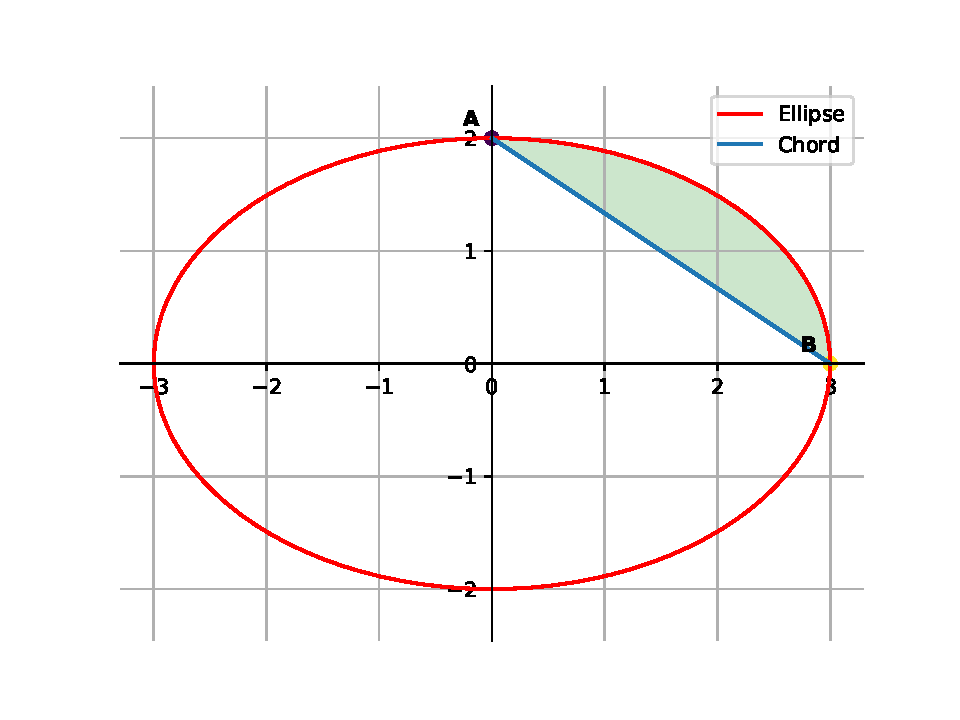
\includegraphics[width=0.75\columnwidth]{chapters/12/8/3/8/figs/fig.pdf}
		\caption{}
		\label{fig:12/8/3/8}
  	\end{figure}
The given ellipse can be expressed as conics with parameters
\begin{align}
\vec{V}=\myvec{
b^2 & 0\\
0 & a^2
},
\vec{u}=0,
f=-(a^2b^2).
\end{align} 
The line parameters are
\begin{align}
\vec{h} &= \myvec{
a\\
0
},
\vec{m} = \myvec{\frac{1}{b} \\ -\frac{1}{a}}.
\end{align}
Substituting the given parameters in \eqref{eq:tangent_roots},
\begin{align}
    \kappa=0,-6
\end{align}
yielding the points of intersection
\begin{align}
    \vec{A}=\myvec{
a\\
0
    },
    \vec{B}=\myvec{
0\\
b
    }.
\end{align}
From 
		\figref{fig:12/8/3/8},
the desired area is
\begin{align}
\int_{0}^{a}\frac{b}{a}\sqrt{a^2-x^2} \,dx 
-\int_{0}^{a} \frac{b}{a}(a-x) \,dx
	= \frac{ab}{2}\brak{\frac{\pi}{2}-1}
	= 3\brak{\frac{\pi}{2}-1}
\end{align}
upon substituting $a=3, b=2$.

\item 
Find the area of the region bounded by the curve $x^2=y$ and the lines $y=x+2$ and the $x$ axis.
\label{chapters/12/8/3/10}
\item 
Find   the area bounded by the curve $y=x|x|, x$-axis and the ordinates $x$=-1 and $x$=1.
\label{chapters/12/8/3/17}
\item 
	Find the area of the region bounded by the curves $y=x^2+2$, $y=x$, $x=0$ and $x=3. $
\label{chapters/12/8/2/3}
\item 
Find the smaller area enclosed by the circle $x^2 + y^2 = 4$ and the line $x + y = 2$. 
\\
\solution
\label{chapters/12/8/2/6}
\begin{enumerate}[label=\thesubsection.\arabic*.,ref=\thesubsection.\theenumi]
\item STATEMENT-1: The curve $y=\frac{-x^2}{2}+x+1$ is symmetric with respect to the line $x=1$.
	\\
STATEMENT-2: A Parabola is symmetric about its axis.
\hfill(2007)
			\begin{multicols}{2}
\begin{enumerate}
    \item Statement-1 is True,Statement-2 is True;Statement-2 is a correct explanation for Statement-1\item  Statement-1 is True,Statement-2 is True;Statement-2 is NOT a correct explanation for Statement-1\item Statement-1 is True,Statement-2 is False\item Statement-1 is False,Statement-2 is True
\end{enumerate}\end{multicols}
\item A parabola has the origin as its focus and $x=2$ as the directrix. Then the vertex of the parabola is at\hfill(2009)
	\begin{multicols}{4}
\begin{enumerate}
    \item $\brak{0,2}$
    \item $\brak{1,0}$
    \item $\brak{0,1}$
    \item $\brak{2,0}$
\end{enumerate}\end{multicols}
\item The ellipse $x^2+y^2 = 4$ is inscribed in a rectangle aligned with the coordinate axes, which in turn is inscribed in another ellipse that passes through the point$\brak{4,0}$. Then the equation of the ellipse is:\hfill(2009)
	\begin{multicols}{2}
\begin{enumerate}
    \item $x^2+12y^2+16$
    \item $4x^2+48y^2=48$
    \item $4x^2+64y^2=48$
    \item $x^2+16y^2=16$
\end{enumerate}\end{multicols}
\item Equation of the ellipse whose axes are the coordinates and which passes through the point $\brak{-3,1}$ and has eccentricity $\sqrt{\frac{2}{5}}$ is\hfill(2011)
	\begin{multicols}{2}
\begin{enumerate}
    \item $5x^2+3y^2-48=0$
    \item $3x^2+5y^2-15=0$
    \item $5x^2+3y^2-32=0$
    \item $3x^2+5y^2-32=0$
\end{enumerate}\end{multicols}
\item An ellipse is drawn by taking a diameter of the circle $(x-1)^2+y^2=1$ as its semi minor axis and a diameter of the circle $x^2+(y-2)^2=4$ as semi-major axis. If the centre of the ellipse is at the origin and its axes are the coordinate axes, then the equation of the ellipse is 

\hfill(2012)
		\begin{multicols}{2}
\begin{enumerate}
    \item $4x^2+y^2=4$ 
    \item $x^2+4y^2=8$
    \item $4x^2+y^2=8$
    \item $x^2+4y^2=1$
\end{enumerate}\end{multicols}
\item The equation of the circle passing through the foci of the ellipse $\frac{x^2}{16}+\frac{y^2}{9}=1$, and having centre at $\brak{0,3}$ is

\hfill( 2013)
			\begin{multicols}{2}
\begin{enumerate}
    \item $x^2+y^2-6y-7=0$
    \item $x^2+y^2-6y+7=0$
    \item $x^2+y^2-6y-5=0$
    \item $x^2+y^2-6y+5=0$
\end{enumerate}\end{multicols}
\item Let $\vec{O}$ be the vertex and $\vec{Q}$ be any point on the parabola, $x^2=8y$. If the point $\vec{P}$ divides the line segment $OQ$ internally in the ratio \brak{1:3}, then the locus of $\vec{P}$ is

\hfill( 2015)
				\begin{multicols}{4}
\begin{enumerate}
    \item $y^2=2x$
    \item $x^2=2y$
    \item $x^2=y$
    \item $y^2=x$
\end{enumerate}\end{multicols}
\item Let $\vec{P}$ be the point on the parabola, $y^2=8x$ which is a minimum distance from the centre $\vec{C}$ of the circle, passing through $\vec{C}$ and having its centre at $\vec{P}$ is

\hfill( 2016)
					\begin{multicols}{2}
\begin{enumerate}
    \item $x^2+y^2-\frac{x}{4}+2y-24=0$ 
    \item $x^2+y^2-4x+9y+18=0$ 
    \item $x^2+y^2-4x+8y+12=0$
    \item $x^2+y^2-x+4y-12=0$
\end{enumerate}\end{multicols}
\item The eccentricity of the hyperbola whose length of the latus rectum is equal to $8$ and the length of its conjugate axis is equal to half of the distance between its foci, is 

\hfill(2016)
						\begin{multicols}{2}
\begin{enumerate}
    \item $\frac{2}{\sqrt{3}}$
    \item $\sqrt{3}$
    \item $\frac{4}{3}$
    \item $\frac{4}{\sqrt{3}}$
\end{enumerate}\end{multicols}

\item Match the conics in column 1 with the statements/expressions in column 2\hfill{(2009)}

\begin{multicols}{2}
\textbf{Column I}
\begin{enumerate}
    \item  Circle
    \item  Parabola
    \item  Ellipse 
    \item  Hyperbola  
\end{enumerate} 
\columnbreak
\textbf{Column II}
\begin{enumerate}
	\item The locus of the point ${(h,k)}$ for which the line $hx + ky =1$ touches the circle $x^2 + y^2 = 4$
    \item Points z in the complex plane satisfying $|z + 2|- |z - 2|= \pm 3$
    \item Points of the conic have parametric representations $x=\sqrt{3}
	    \brak{\frac{1 - t^2}{1 + t^2}}$, $ y = \frac{2t}{1 + t^2}$

    \item The eccentricity of the conic lies in the interval $1 \leq x < \infty$

\end{enumerate}
\end{multicols}


 \item Let $H : \frac{x^2}{a^2}-\frac{y^2}{b^2}= 1$, where $a>b>0$, be a hyperbola in $XY$-plane whose conjugate axis $LM$ subtends an angle of $60\degree$ at one of its vertices $\vec{N}$. Let the area of the triangle $LMN$ be 4$\sqrt{3}$.
Match the following.
\begin{multicols}{2}
\textbf{List 1}
\begin{enumerate}
    \item The length of the conjugate axis of $H$ is
    \item The eccentricity of $H$ is
    \item The distance between the foci of $H$ is
    \item The length of the latus rectum of $H$ is
\end{enumerate}
\columnbreak
\textbf{List 2}
\begin{enumerate}
    \item 8
    \item $\frac{4}{\sqrt{3}}$
    \item $\frac{2}{\sqrt{3}}$
    \item 4
\end{enumerate}
\end{multicols}
\item If $\vec{P}=\brak{x,y}$, $\vec{F}_{1}=\brak{3,0}$, $\vec{F}_{2}=\brak{-3,0}$ and $16x^2+25y^2=400$, then ${PF}_{1}+{PF}_{2}$ equals \hfill(1998)
	\begin{multicols}{4}
	\begin{enumerate}
		\item $8$
		\item $6$
		\item $10$
		\item $12$
	\end{enumerate}\end{multicols}

\item Let a hyperbola passes through the focus of the ellipse $\frac{x^2}{25}+\frac{y^2}{16}=1$. The transverse and conjugate axes of this hyperbola coincide with the major and minor axes of the given ellipse, also the product of eccentricities of given ellipse and hyperbola is $1$, then \hfill (2006)
	\begin{multicols}{2}
	\begin{enumerate}
		\item the equation of hyperbola is $\frac{x^2}{9}-\frac{y^2}{16}=1$
		\item the equation of hyperbola is $\frac{x^2}{9}-\frac{y^2}{25}=1$
		\item focus of hyperbola is $\brak{5,0}$
		\item vertex of hyperbola is $\brak{5\sqrt{3},0}$
	\end{enumerate}\end{multicols}

\item Let $\vec{P}\brak{x_{1}, y_{1}}$ and $\vec{Q}\brak{x_{2},y_{2}}$, $y_{1}<0,y_{2}<0$, be the end points of the latus rectum of the ellipse $x^2+4y^2=4$. The equations of parabolas with latus rectum ${PQ}$ are \hfill(2008)
	\begin{multicols}{2}
	\begin{enumerate}
		\item $x^2+2\sqrt{3}y=3+\sqrt{3}$
		\item $x^2-2\sqrt{3}y=3+\sqrt{3}$
			\columnbreak
		\item $x^2+2\sqrt{3}y=3-\sqrt{3}$
		\item $x^2-2\sqrt{3}y=3-\sqrt{3}$
	\end{enumerate}\end{multicols}

\item In a triangle ${ABC}$ with fixed base ${BC}$, the vertex $\vec{A}$ moves such that
	$$\cos{B}+\cos{C}=4\sin^2{\frac{A}{2}}.$$
		If $a,b$ and $c$ denote the lengths of the sides of the triangle opposite to the angles $A,B$ and $C$, respectively, then \hfill(2009)\\
		\begin{enumerate}
			\item $b+c=4a$
			\item $b+c=2a$
			\item locus of the point $\vec{A}$ is an ellipse
			\item locus of the point $\vec{A}$ is a pair of straight lines
		\end{enumerate}

	\item Let the eccentricity of the hyperbola $\frac{x^2}{a^2}-\frac{y^2}{b^2}=1$ be reciprocal to that of the elipse $x^2+4y^2=4$. If the hyperbola
	passes through a focus of the elipse, then 
		\hfill(2011)
		 \begin{enumerate}
			\item the equation of the hyperbola is $\frac{x^2}{3}-\frac{y^2}{2}=1$
			\item a focus of the hypebola is $(2,0)$
			\item the eccentricity of the hyperbola is $\sqrt{\frac{5}{3}}$
			\item the equation of the hyperbola is $x^2-3y^2=3$
		 \end{enumerate}
	\item Let $\vec{P}$ and $\vec{Q}$ be distinct points on the parabola $y^2=2x$ such 
		that a circle with $PQ$ as diameter passes through the vertex
		$\vec{O}$ of the parabola. If $\vec{P}$ lies in the first quadrant and the area
		of the triangle  \(\Delta \)$OPQ$ is 3$\sqrt{2}$, then which of the following is
		(are) the coordinates of $\vec{P}$?  
		\hfill(2015)
				\begin{multicols}{4}
		 \begin{enumerate}
			\item $ \brak{4,2\sqrt{2}}$
			\item $\brak{9,3\sqrt{2}}$
			\item $ \brak{\frac{1}{4},\frac{1}{\sqrt{2}}}$
			\item  $ \brak{1,\sqrt{2}}$
		 \end{enumerate}\end{multicols}
    \item The equation $\frac{x^2}{1-r}-\frac{y^2}{1+r}=1,r > 1$
represents
          \hfill  \brak{1981}
					\begin{multicols}{2}
\begin{enumerate}
    \item an ellipse    \item       a hyperbola
   \item a circle     \item    none of there 
\end{enumerate}\end{multicols}
\item Each of the four inequalities give below defines a region in $xy$ plane.One of these four regions does not have the following property.For any two points   $\brak{\frac{x_1+x_2}{2},\frac{y_1+y_2}{2}}$   is also in region.The inequality defining this region is:
         \hfill \brak{1981}
						\begin{multicols}{2}
\begin{enumerate}
    \item $x^2+2y^2\le1$
    \item Max $\abs{x},\abs{y}$ $\le1$
    \item $x^2-y^2\le1$
    \item $y^2-x\le0$
\end{enumerate}\end{multicols}
\item The equation $2x^2+3y^2-8x-18y+35=k$ represents
        \hfill \brak{1994}
							\begin{multicols}{2}
\begin{enumerate}
    \item no locus if $k\textless0$
    \item an ellipse if $k\textless0$
    \item a point if $k=0$
    \item a hyperbola if $k\textgreater0$ 
\end{enumerate}\end{multicols}
\item Let $E$ be the ellipse $\frac{x^2}{9}+\frac{y^2}{4}=1$ and $C$ be the circle $x^2+y^2=9$. Let $\vec{P}$ and $\vec{Q}$ be the points $\brak{1,2}$ and $\brak{2,1}$ respectively.Then
        \hfill \brak{1994}
								\begin{multicols}{2}
\begin{enumerate}
    \item $\vec{Q}$ lies inside $C$ but outside $E$
    \item $\vec{Q}$ lies outside both $C$ and $E$
    \item $\vec{P}$ lies inside both $C$ and $E$
    \item $\vec{P}$ lies inside $C$ but outside $E$ 
\end{enumerate}\end{multicols}
\item The radius of the circle passing through the foci of the ellipse $\frac{x^2}{16}+\frac{y^2}{9}=1$ and having its centre at $\brak{0,3}$ is
       \hfill \brak{1995}
									\begin{multicols}{4}
\begin{enumerate}
    \item $4$
    \item $3$
    \item $\sqrt{\frac{1}{2}}$
    \item $\frac{7}{2}$
\end{enumerate}\end{multicols}
\item The curve described parametrically by $x=t^2+t+1$, $y=t^2-t+1$ represents
     \hfill\brak{1999}
										\begin{multicols}{2}
\begin{enumerate}
    \item a pair of straight lines
    \item an ellipse
    \item a parabola
    \item a hyperbola
\end{enumerate}\end{multicols}
\item If the line $x-1=0$ is the directrix of parabola $y^2-kx+8=0$, then one of the values of $K$ is
      \hfill\brak{2000}
											\begin{multicols}{2}
\begin{enumerate}
    \item $\frac{1}{8}$
    \item $8$
    \item $4$
    \item $\frac{1}{4}$ 
\end{enumerate}\end{multicols}
    \item The equation of the directrix of the parabola $y^2+4y+4x+2=0$ is 
     \hfill \brak{2001}
												\begin{multicols}{2}
\begin{enumerate}
    \item $x=-1$
    \item $x=1$
    \item $x=-\frac{3}{2}$
     \item $x=\frac{3}{2}$
\end{enumerate}\end{multicols}
\item The locus of the mid-point of the line segment joining the focus to a moving point on the parabola $y^{2} = 4ax$ is another parabola with directrix \hfill{(2002)}
\begin{multicols}{4}
 \begin{enumerate}
    \item x=-a
    \item x=-a/2
    \item x=a
    \item x=a/2
 \end{enumerate}
\end{multicols}
\item For hyperbola $\frac{x^{2}}{\cos^{2}\alpha}-\frac{y^{2}}{\sin^{2}\alpha}=1$ which of the following remains constant with change in $\alpha$
\hfill{(2003)}
\begin{multicols}{2}
\begin{enumerate}
    \item abscissae of vertices
    \item abscissae of foci
    \item eccentricity
    \item directrix
\end{enumerate}
\end{multicols}
\item The axis of the parabola is along the line $y=x$ and the distance of its vertex and focus from  origin are $\sqrt2$ and $2\sqrt2$  respectively. If the vertex and focus both lie in the first quadrant,then the equation of the parabola is \hfill{(2006)}
\begin{multicols}{2}
\begin{enumerate}
    \item $(x+y)^{2}=(x-y-2)$
    \item $(x-y)^{2}=(x+y-2)$
    \item $(x-y)^{2}=4(x+y-2)$
    \item $(x-y)^{2}=8(x+y-2)$
\end{enumerate}
\end{multicols}
\item A hyperbola, having the transverse axis of length $2\sin\theta$, is confocal with the ellipse $3x^{2}+4y^{2}=12$. Then its equation is \hfill{(2007)}
	\begin{multicols}{2}
\begin{enumerate}
    \item ${x^{2}\cosec^{2}\theta}-{y^{2}\sec^{2}\theta=1}$
    \item $x^{2}\sec^{2}\theta-y^{2}\cosec^{2}\theta=1$
    \item $x^{2}\sin^{2}\theta-y^{2}\cos^{2}\theta=1$
    \item $x^{2}\cos^{2}\theta-y^{2}\sin^{2}\theta=1$
\end{enumerate}\end{multicols}
\item Let $a$ and $b$ be non-zero real numbers. Then, the equation $(ax^{2}+by^{2}+c)(x^{2}-5xy+6y^{2}=0)$ represents \hfill{(2008)}
\begin{enumerate}
    \item four straight lines, when $c=0$ and $a, b$ are of the same sign.
    \item two straight lines and a circle, when $a=b$,and $c$ is of sign opposite to that of $a$.
    \item two straight lines and a hyperbola, when $a$ and $b$ are of the same sign and $c$ is of opposite to that of $a$.
    \item a circle and an ellipse, when $a$ and $b$ are of the same sign and $c$ is of sign opposite to that of $a$.
\end{enumerate}
\item Consider a branch of the hyperbola $x^{2}-2y^{2}-2\sqrt{2}x-4\sqrt{2}y-6=0$ with vertex at a point  $\vec{A}$. Let  $\vec{B}$  be one of the end points of its latus rectum. If $\vec{C}$ is the focus of the hyperbola nearest to the point  $\vec{A}$, then the area of the triangle $ABC$ is \hfill{(2008)}
\begin{multicols}{4}
\begin{enumerate}
    \item $1-\sqrt{\frac{2}{3}}$
    \item $\sqrt{\frac{3}{2}}-1$
    \item $1+\sqrt{\frac{2}{3}}$
    \item $\sqrt{\frac{3}{2}}+1$
\end{enumerate}
\end{multicols}
\item The line passing through the extremity $\vec{A}$ of the major axis and extremity $\vec{B}$ of the minor axis of the ellipse $x^{2}+9y^{2}=9$ meets its auxillary circle at the point $\vec{M}$. Then the area of the triangle with the vertices at $\vec{A}$, $\vec{M}$ and the origin $\vec{O}$ is \hfill{(2009)}
\begin{multicols}{4}
\begin{enumerate}
    \item $\frac{31}{10}$
    \item $\frac{29}{10}$
    \item $\frac{21}{10}$
    \item $\frac{27}{10}$
\end{enumerate}\end{multicols}
	%	
\item The locus of the orthocentre of the triangle formed by the lines
		
			$$\brak{1+p}x-py+p\brak{1+p}=0,$$
			$$\brak{1+q}x-qy+q\brak{1+q}=0,$$
		and $y=0$, where $p \neq q$, is
		\hfill(2009)
		\begin{multicols}{4}
\begin{enumerate}
	\item a hyperbola
	\item a parabola
	\item an ellipse
	\item a straight line
\end{enumerate}\end{multicols}
%
	\item Let $\brak{x,y}$ be any point on the parabola $y^2=4x$. Let $\vec{P}$ be the point that divides the line segment from $\brak{0,0}$ to $\brak{x,y}$ in the ratio $1:3$. Then the locus of $\vec{P}$ is  \hfill(2011)
		\begin{multicols}{4}
		\begin{enumerate}
			\item $x^2=y$
			\item $y^2=2x$
				\columnbreak
			\item $y^2=x$
			\item $x^2=2y$
		\end{enumerate}\end{multicols}
%
	\item The ellipse $E_{1}$:$\frac{x^2}{9}+\frac{y^2}{4}=1$ is inscribed in a rectangle $\vec{R}$ whose sides are parallel to the coordinate axes. Another ellipse $E_{2}$ passing through the point $\brak{0,4}$ circumscribes the rectangle $\vec{R}$. The eccentricity of the ellipse $E_{2}$ is \hfill(2012)
%
		\begin{multicols}{4}
		\begin{enumerate}
			\item $\frac{\sqrt{2}}{2}$
			\item $\frac{\sqrt{3}}{2}$
				\columnbreak
			\item $\frac{1}{2}$
			\item $\frac{3}{4}$
		\end{enumerate}\end{multicols}
%
\item  Two sets $A$ and $B$ are as under:
$A=\cbrak{\brak{a,b}\in\mathbb{R}\times\mathbb{R}:\abs{a-5}<1\text{ and} \abs{b-5}<1}$
$B=\cbrak{\brak{a,b}\in\mathbb{R}\times\mathbb{R}:4(a-6)^2\text{+}9(b-5)^2\leq36}$
    \hfill{( 2018)}
			\begin{multicols}{2}
	\begin{enumerate}
		\item $A\subset B$ 
		\item $A\cap B$
		\item neither $A\subset B$ nor $B\subset A$
		\item $B\subset A$
	\end{enumerate}\end{multicols}
\item Axis of a parabola lies along $X$ axis. If its vertex and focus are at a distance $2$ and $4$ respectively from origin, on the positive $X$ axis then which of the following points does not lie on it? 
     \hfill{( 2018)} 
				\begin{multicols}{4}
	\begin{enumerate}
    		\item $\brak{5,2\sqrt6}$
    		\item $\brak{8,6}$
    		\item $\brak{6,4\sqrt2}$
    		\item $\brak{4,-4}$
	\end{enumerate}\end{multicols}
\item Let $0<\theta<\pi/2$. If the eccentricty of the hyperbola $\frac{x^2}{\cos^2{\theta}} - \frac{y^2}{\sin^2{\theta}} = 1$ is greater than $2$, then the length of its latus rectum lies in the interval
	\hfill{( 2019)}
					\begin{multicols}{4}
	\begin{enumerate}
    		\item $\brak{5,\infty}$
    		\item $\lbrak{\frac{3}{2}},\rsbrak{3}$
    		\item $\lbrak{2},\rsbrak{3}$ 
    		\item $\lbrak{1},\rsbrak{\frac{3}{2}}$
	\end{enumerate} \end{multicols}
\item  The equation of the locus of the point whose distances from the point $\Vec{P}$ and the line $AB$ are equal, is

	\begin{multicols}{2}
\begin{enumerate}
     \item $9x^2+y^2-6xy-54x-62y+241=0$
     \item $x^2+9y^2+6xy-54x-62y-241=0$
     \item $9x^2+9y^2-6xy-54x-62y-241=0$
     \item $x^2+y^2-2xy+27x+31y-120=0$
\end{enumerate}\end{multicols}
\item Let $\vec{P}$ be a point on the ellipse $\frac{x^2}{a^2}+\frac{y^2}{b^2}=1$, $0<b<a$. Let the line parallel to the $X$ axis passing through $\vec{P}$ meet the circle $x^2+y^2=a^2$ at the point $\vec{Q}$ such that $\vec{P}$ and $\vec{Q}$ are on the same side of the $X$ axis. For two positive real numbers $r$ and $s$, find the locus of the point $\vec{R}$ on $PQ$ such that $PR
= r$ as $\vec{P}$ varies over the ellipse. \hfill\brak{2001}


	\end{enumerate}

\item Find the area of the region bounded by the curves $y^2 = 9x$, $y = 3x$.
\item Find the area of the region bounded by the parabola $y^2 = 2px$, $x^2 = 2py$.
\item Find the area of the region bounded by the curve $y = x^2\text{ and }y = x + 6\text{ and }x = 0$.
\item Find the area of the region bounded by the curve $y^2 = 4x$, $x^2 = 4y$.
\item Find the area of the region included between $y^2 = 9x\text{ and }y =x$
\item Find the area of the region enclosed by the parabola $x^2 = y$ and the line $y = x + 2$
\item Find the area of region bounded by the line $x = 2$ and the parabola $y^2 = 8x$
\item Sketch the region ${(x,0) : y = \sqrt{4 - x^2}}$ and $x$-axis. Find the area of the region using integration.
\item Calculate the area under the curve $y = 2\sqrt{x}$ included between the lines $x = 0\text{ and }x = 1$.
\item Using integration, find the area of the region bounded by the line $2y = 5x + 7$, $x$-axis and the lines $x = 2\text{ and }x =8$.
\item Draw a rough sketch of the curve $y = \sqrt{x - 1}$ in the interval $[1, 5]$. Find the area under the curve and between the lines $x = 1\text{ and }x = 5$.
\item Determine the area under the curve $y = \sqrt{a^2 - x^2}$ included between the lines $x = 0\text{ and }x = a$
\item Find the area of the region bounded by $y = \sqrt{x}\text{ and }y = x$.
\item Find the area enclosed by the curve $y = - x^2$ and the straight line $x + y + 2 = 0$.
\item Find the area bounded by the curve $y = \sqrt{x}$, $x = 2y + 3$ in the first quadrant and $x$-axis.
\item Draw a rough sketch of the region ${(x, y) : y^2 \lessgtr 6ax\text{ and }x^2 + y^2 \lessgtr 16a^2}$.
\item Draw a  rough sketch of the given curve $y =1 + \abs{x + 1}$, $x = -3$, $x = 3$, $y = 0$, and find the area of the region bounded by them, using integration.
\item The area of the region bounded by the curve $x^2 = 4y$ and the straight line $x = 4y - 2$ is
\begin{enumerate}
\item $\frac{3}{8}$ sq units 
\item $\frac{5}{8}$ sq units
\item $\frac{7}{8}$ sq units 
\item $\frac{9}{8}$ sq units
\end{enumerate}
\item The area of the region bounded by the curve $y = \sqrt{16 - x^2}$ and $x$-axis is 
\begin{enumerate}
\item 8 sq units 
\item ${20\pi}$ sq units
\item ${16\pi}$ sq units
\item ${256\pi}$ sq units
\end{enumerate}
\item Area of the region in the first quadrant enclosed by the $x$-axis, the line $y = x$ and the circle $x^2 + y^2 = 32$ is 
\begin{enumerate}
\item ${16\pi}$ sq units 
\item ${4\pi}$ sq units
\item ${32\pi}$ sq units
\item ${24\pi}$ sq units
\end{enumerate}
\item The area of the region bounded by parabola $y^2 = x$ and the straight line $2y = x$ is
\begin{enumerate}
\item $\frac{4}{3}$ sq units
\item 1 sq units
\item $\frac{2}{3}$ sq units 
\item $\frac{1}{3}$ sq units
\end{enumerate}
\item Find the equation of a circle whose centre is (3,1) and which cuts off a chord of length  6 units on the  line $2x-5y+18=0$.
\end{enumerate}
